\documentclass[techreport]{IEEEtran}
\usepackage{cite}
\usepackage{amsmath,amssymb,amsfonts}
\usepackage{algorithmic}
\usepackage{graphicx}
\usepackage{textcomp}
\usepackage{xcolor}
\usepackage{listings}
\usepackage{float}
\usepackage[spanish,mexico]{babel}

\usepackage{caption}
\usepackage{subcaption}

\usepackage{import}
\usepackage{xifthen}
\usepackage{pdfpages}
% \usepackage{multicol}
% \usepackage{transparent}

\graphicspath{{img/}}

\DeclareMathOperator{\atantwo}{atan2}

\DeclareMathOperator{\arctantwo}{arctan2}

\def\BibTeX{{\rm B\kern-.05em{\sc i\kern-.025em b}\kern-.08em
    T\kern-.1667em\lower.7ex\hbox{E}\kern-.125emX}}
    
\begin{document}

\title{
Análisis, simulación y comparación de gastos energéticos de la plataforma Gough-Cappel con distintos modelos de control\\
}


\author{
    \IEEEauthorblockN{
    Enrique Benavides Téllez, 
    Isaac Ayala Lozano y 
    Neftali Jonatán González Yances\\
    }
    \IEEEauthorblockA{
    \textit{Robótica y Manufactura Avanzada} \\
    \textit{CINVESTAV}\\
        Ramos Arizpe, México}
}

\maketitle

\begin{abstract}
Se presenta la comparación energética de tres estrategias de control en lazo cerrado para la plataforma Gough-Cappel.
Se describe el desarrollo matemático del sistema y la implementación del mismo en MATLAB.
\end{abstract}

% % \begin{IEEEkeywords}
% \end{IEEEkeywords}


Uno de los manipuladores paralelos mas populares es la \emph{Plataforma Gough-Stewart} (PGS) de 6 gdl (grados de libertad) propuesto por Eric Gough en 1954 y mejorado por D. Stewart en 1965 con la intención de realizar un simulador de vuelo como una de las aplicaciones finales de la plataforma. El sistema consiste en una plataforma movil, una plataforma fija y seis brazos extensibles conectando las dos plataformas. \\
\\
Una estructura paralelea es considerada una cadena cinemática cerrada, los brazos están conectados del efector final al origen por medio de una conexión paralela. El desarrollo cinemático del sistema es complicado y para su solución se necesita del entendimiento general de la PGS y su forma de operación. La cinemática de un robot se puede dividir entre cinemática directa e inversa. La cinemática directa se centra en encontrar la posicion y orientación del efector final al modificar las dimensiones de los brazos y la cinemática inversa se centra en utilizar la posicion final del efector final para encontrar el valor longitudinal de los brazos.El desarrollo de la cinemática inversa de la PGS es sencilla de obtener, sin embargo el desarrollo de la cinemática directa es complicada debido a la necesidad de solucionar ecuaciones no lineales para la solución. \\
\\
De la misma forma, es necesario conocer el modelo dinámico del sistema el cual define la menra en la que las energías y fuerzas se comportan en el sistema y contiene al igual que la cinemática directa complicaciones de desarrollo debido a la estructura de ciclo cerrado y las relaciones entre las partes del sistema. El modelo dinámico puede ser obtenido por medio de alguno de los siguientes métodos: \emph{Euler-Lagrange, principio de trabajo virtual, D'Alembert-Lagrange}.
Para fines del documento se utilizará el método de D'Alembert-Lagrange para obtener el modelo dinámico de la PGS. 
Cualquier robot para poder tener la fuerza y precisión para realizar una acción debe de poder rechazar perturbaciones externas asi como mantener la estabilidad en una referencia deseada, inclusive  si la referencia está en constante cambio. La teoría de control propone diferentes maneras de llegar a la estabilidad por medio de la aplicación de gradientes de energía suficientes para mantener la estabilidad en la referencia deseada.\\
\\

Por medio del presente escrito definirá en un inicio la cinemática de la PGS y seguido se realizará el modelo dinámico de la plataforma. En el aparatdo III se observarán los resultados del modelo dinámico con dos diferentes leyes de control (PD y PID) para comparar el gasto energético de cada uno con respecto a la tarea que debe realizar el robot.


% \section{Marco Teórico}

\subsection{Mecánica Lagrangiana}

asd

\subsection{Formulación de Kirchhoff para la dinámica de un cuerpo rígido}

De

% \section{Desarrollo}
\section{Parámetros de diseño}

\subsection{Restricciones}
El robot paralelo está restringido en su movimiento 
al ser una cadena cerrada.
A su vez, el diseño del mismo impone restricciones dimensionales 
que deben ser tomadas en cuenta para su análisis.
Estas restricciones surgen de los parámetros de diseño que 
se seleccionaron para el modelo del robot y el simulador.
La tabla \ref{tab: restricciones} muestra los 
parámetros de diseño establecidos.

\begin{figure}
 \centering
 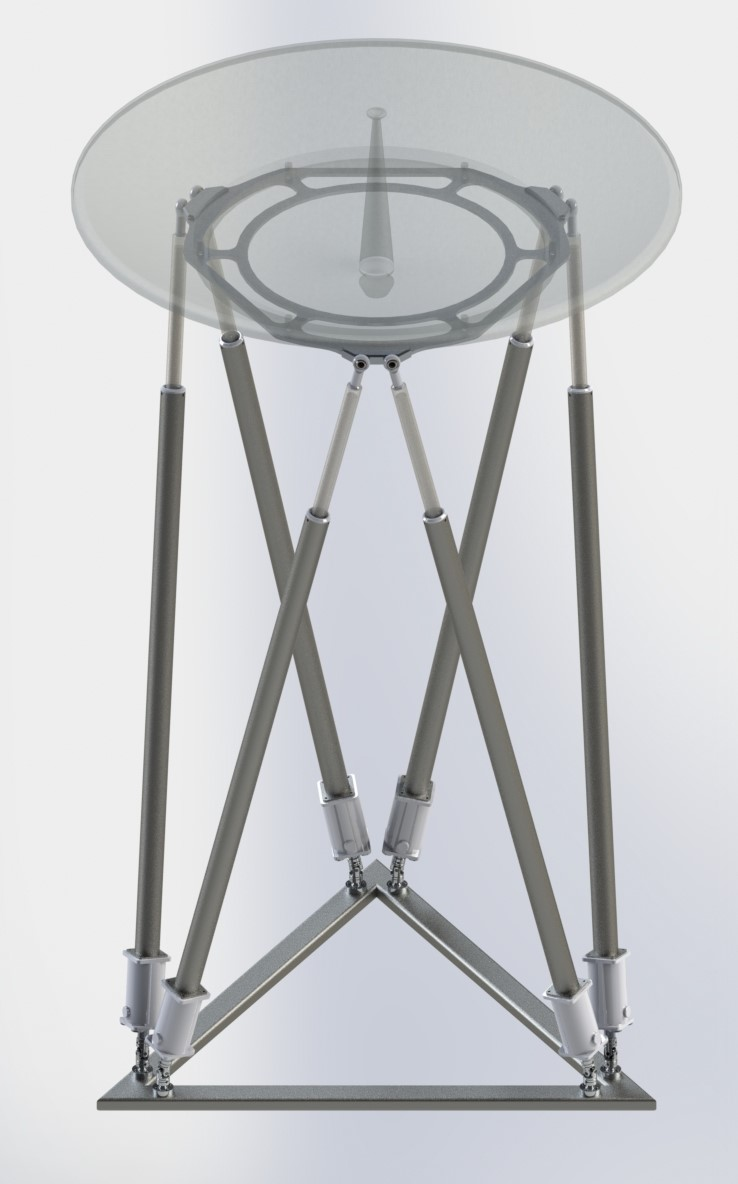
\includegraphics[width=8.5cm]{PGScrop.jpg}
 \caption{Plataforma Gough-Cappel.}
 \label{fig: cad}
\end{figure}


\begin{table}[htb!]
\centering
\begin{tabular}{lc}

\multicolumn{2}{c}{Parámetros de diseño} \\ \hline
Radio de la base ($r_b$) & $0.44205 \ [m]$ \\ 
Radio de la plataforma ($r_a$) & $0.36248 \ [m]$ \\ 
Separación entre juntas en la base ($k_b$) & $0.7 \ [m]$ \\ 
Separación entre juntas en la plataforma ($k_a$) & $0.2986 \ [m]$ \\ 
Longitud mínima del actuador ($q_{min}$) & $1.28929 \ [m]$ \\ 
Mangitud máxima del actuador ($q_{max}$) &  $2.19 \ [m]$ \\ 
\end{tabular}
\caption{Restricciones dimensionales del robot paralelo.}
\label{tab: restricciones}
\end{table}

Las restricciones presentes en la tabla \ref{tab: restricciones}
son utilizados para definir la cinemática del robot paralelo.
Los valores de $r_a$ y $r_b$ definen la 
distancia radial en la que cada junta debe ser 
posicionada respecto al centro de la plataforma y la base.
Las juntas empleadas para el robot se muestran 
en la figura \ref{fig: joints}

\begin{figure}[htb!]
 \centering
    \begin{subfigure}[b]{0.4\textwidth}         
    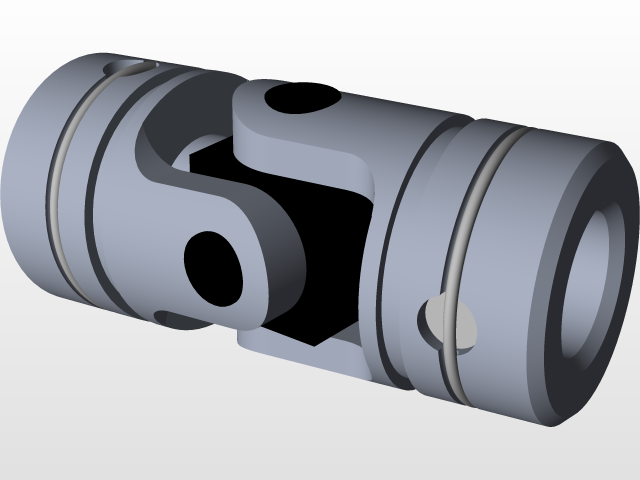
\includegraphics[width=\textwidth]{CARDAN.png}
        \caption{Junta universal o cardán.}
        \label{fig: junta universal}
    \end{subfigure}
    
    ~ %add desired spacing between images, e. g. ~, \quad, \qquad, \hfill etc. 
      %(or a blank line to force the subfigure onto a new line)
    \begin{subfigure}[b]{0.4\textwidth}
         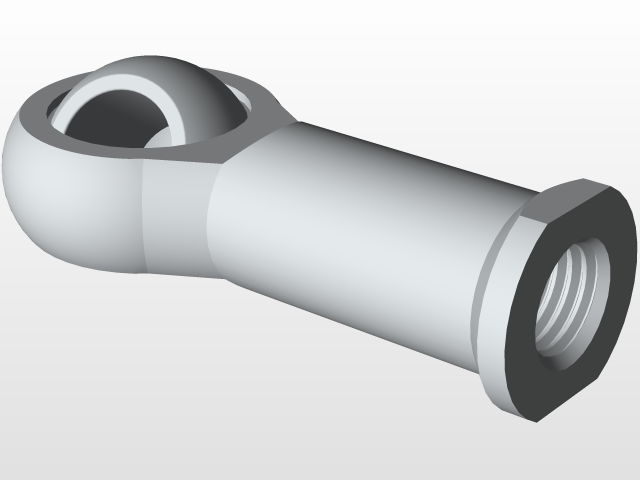
\includegraphics[width=\textwidth]{BALL_JOINT.png}
        \caption{Junta esférica.}
        \label{fig: junta esferica}
    \end{subfigure}
    ~ %add desired spacing between images, e. g. ~, \quad, \qquad, \hfill etc. 
    %(or a blank line to force the subfigure onto a new line)
    \caption{Juntas empleadas en la plataforma Gough-Cappel}\label{fig: joints}
\end{figure}

Las junta universales (figura \ref{fig: junta universal}) están
instaladas en la base del robot. 
La junta universal permite rotaciones en dos ejes.
La configuración de las juntas determina el orden de las rotaciones.
Para el robot diseñado se presenta una rotación en el eje y primero.
Una rotación en el eje x ocurre despúes de la primer rotación.
La orientación de las juntas establece que el eje y 
del marco referencial local se oriente en dirección al centro de la base.

Las juntas esféricas (figura \ref{fig: junta esferica}) conectan la 
plataforma móvil con los actuadores prismáticos.
Estas juntas permiten rotaciones en los tres ejes del marco referencial
local.
El orden de las rotaciones se asigna de la siguiente manera:
primero una rotación en el eje z, seguido de la rotación del 
marco referencial en el eje x, y finalmente el marco 
referencial es rotado en y.

\subsection{Ángulos de desfase}

La ubicación ideal de las juntas en la base y la plataforma móvil 
es en tres puntos ubicados sobre los radios $r_a$ y $r_b$, 
a 120 grados de distancia angular de cada uno, 
cada punto siendo la ubicación de dos juntas.
Las restricciones del modelo real del robot paralelo no permiten esta
ubicación, ya que esta posición no considera las posibles obstrucciones
que cada componente puede tener sobre los otros.\\

A manera de evitar estas obstrucciones y las posibles 
colisiones que conllevarían, 
las distancias $k_a$ y $k_b$ son parámetros de diseño.
Estas distancias generan ángulos de desfase 
$\alpha_a$ y $\alpha_b$ respecto al ángulo ideal de ubicación.
Estos ángulos de desfase son calculados de la siguiente manera:

\begin{equation} \label{eq: azi-a}
\alpha_a = \arctan\left(\frac{k_a}{2r_a}\right)
\end{equation}
\begin{equation} \label{eq: azi-b}
\alpha_b = \arctan\left(\frac{k_b}{2r_b}\right)
\end{equation}

Los ángulos de desfase permiten determinar las nuevas posiciones angulares 
$\Psi$ de cada junta, tal que la distancia angular de cada par de juntas 
respecto a su posición ideal sea $\pm \alpha$. 
Determinando los valores de $\psi_a$ y $\psi_b$, es posible
obtener los vectores de posición $\mathbf a_i$ y $\mathbf b_i$ 
para el punto de unión de cada junta
medido respecto a los marcos referenciales locales de 
la base ($\Sigma_b$) y la plataforma móvil ($\Sigma_a$).


\begin{equation} \label{eq: p_b}
\mathbf b_i = \begin{bmatrix}
r_b\cos(\psi_{bi})\\
r_b\sin(\psi_{bi})\\
0\\
\end{bmatrix}
\end{equation}

\begin{equation} \label{eq: p_a}
\mathbf a_i = \begin{bmatrix}
r_a\cos(\Psi_{ai})\\
r_a\sin(\Psi_{ai})\\
0\\
\end{bmatrix}
\end{equation}

\section{Cinemática}

La cinemática del robot paralelo es obtenida del conocimiento de una posición $\mathbf d$
y una orientación $\mathbf \theta_p$ deseada del efector final.
La posición de la plataforma móvil está dada por el vector $\mathbf p = [x \ y \ z]^T$
La orientación es el vector $\boldsymbol \theta_p = [\psi \ \theta \ \phi]^T$, 
cuyos elementos son los ángulos de la plataforma medidos respect al marco referencial inercial.

\begin{figure}[htb!]
    \centering
    \import{./img/}{isometric.pdf_tex}
%     \import{./img/}{goughStewart.pdf_tex}
    \caption{Diagrama de la plataforma Gough-Cappel.}
    \label{fig: gough stewart diagram}
\end{figure}

\subsection{Cinemática inversa de posición}

La cinemática inversa del robot paralelo parte de la suma de vectores 
mostrados en la figura \ref{fig: gough stewart diagram}.
Se observa que el vector de posición $\mathbf p_i$ puede ser representado 
por dos sumas equivalentes. 
\begin{itemize}
 \item La suma del vector de posición de la plataforma $\mathbf d$ 
medido respecto al referencial inercial y el producto de 
la matriz de rotación extrínseca $\mathbf R$ y el vector de posición 
de la junta $\mathbf a_i$. 
 \item La suma del vector de posición $\mathbf l_i$ medido respecto 
 al referencial local de la junta y el vector de posición $\mathbf b_i$.
\end{itemize}

\begin{subequations} \label{eq: plat_grl}
 \begin{align}
    \mathbf p_i & = \mathbf d + \mathbf R\mathbf a_i \\
    \mathbf p_i & = \mathbf b_i + \mathbf l_i
 \end{align}
\end{subequations}


Los elementos de la matriz de rotación 
extrínseca $\mathbf R$ están en función del vector $\mathbf \theta_p$.
La matriz se representa de la siguiente manera:

\begin{equation} \label{eq: Mrot-P}
\mathbf R = \begin{bmatrix}
C_\psi C_\theta & -S_\psi C_\phi + C_\psi S_\theta S_\phi & S_\psi S_\phi + C_\psi S_\theta C_\phi\\
S_\psi C_\theta & C_\psi C_\phi + S_\psi S_\theta S_\phi & -C_\psi S_\phi + S_\psi S_\theta C_\phi\\
-S_\theta & C_\theta S_\phi & C_\theta C_\phi\\
\end{bmatrix}
\end{equation}

El movimiento de la plataforma es determinado por el cambio de longitud
de los actuadores prismáticos $||\mathbf l_i||$.
Esta característica del sistema permite establecer
a las longitudes de los actuadores como las coordenadas 
generalizadas $q_i$ del sistema.
Cada coordenada generaliza se define entonces como la norma euclidiana
del vector $\mathbf l_i$ correspondiente.
A su vez, el vector $\mathbf l_i$ se obtiene al resolver 
\eqref{eq: plat_grl}.

\begin{equation} \label{eq: coord_grl}
    q_i = ||\mathbf l_i||
\end{equation}

\begin{equation} \label{eq: l}
    ||\mathbf l_i|| = \sqrt{<\mathbf l_i, \mathbf l_i>} 
\end{equation}

\begin{equation} \label{eq: largo_act}
\mathbf l_i = \mathbf d + \mathbf R \mathbf a_i - \mathbf b_i
\end{equation}

Utilizando las ecuaciones \ref{eq: coord_grl} y 
\ref{eq: largo_act} se obtiene el vector unitario 
$\boldsymbol \lambda_i$.

\begin{equation} \label{eq: vec_U}
\boldsymbol \lambda_i = \frac{\mathbf l_i}{q_i}
\end{equation}

\subsection{Pseudocinemática directa}

Para la obtención de la cinemática directas se propone la división de cada cadena paralela en 
cadenas seriales partiendo del marco referencial inercial.
A cada junta se asignan referenciales de movimiento rotacional  en sus
respectivos ejes.
Esto permite el cálculo de cada cadena serial mediante 
transformaciones homogéneas (figura \ref{fig: cadena serial}).
Esta propuesta permite obtener un resultado fiable a pesar de la 
complejidad que presenta la obtención de la 
cinemática directa del sistema.

\begin{figure}[htb!]
 \centering
 \import{./img/}{frames.pdf_tex}
 \caption{Referenciales de la cadena serial.}
 \label{fig: cadena serial}
\end{figure}

Las transformaciones homogéneas $H_{ij}$ se presentan a
continuación:

\begin{subequations}
 \begin{align}
%   \sum_0^1 
  H_{i0} & = \begin{bmatrix}
R_z(\Psi_{bi}) & b_i\\
0 & 1
\end{bmatrix} \\
% \sum_1^2 
H_{i1} & = \begin{bmatrix}
R_y(\theta_{1i}) & 0\\
0 & 1
\end{bmatrix} \\
% \sum_2^3
H_{i2} & = \begin{bmatrix}
R_x(\theta_{2i}) & 0\\
0 & 1
\end{bmatrix} \\
% \sum_3^4 
H_{i3} & = \begin{bmatrix}
I_3 & q_{min}\\
0 & 1
\end{bmatrix}\\
% \sum_4^5
H_{i4} & = \begin{bmatrix}
R_z(\theta_{4i}) & l_i\\
0 & 1
\end{bmatrix} \\
% \sum_4^5 
H_{i5} & = \begin{bmatrix}
R_x(\theta_{5i}) & 0\\
0 & 1
\end{bmatrix} \\
% \sum_5^6 
H_{i6} & = \begin{bmatrix}
R_y(\theta_{6i}) & 0\\
0 & 1
\end{bmatrix} \\
% \sum_6^7
H_{i7} & = \begin{bmatrix}
R_z(\Psi_{ai}) & -Ra_i\\
0 & 1
\end{bmatrix}
 \end{align}
\end{subequations}

\begin{equation}
 \Psi_{bi}  = \psi_{bi} + \pi/2
\end{equation}

\begin{equation}
 \Psi_{ai}  = \psi_{ai} - \pi/2
\end{equation}

\subsection{Pseudocinemática inversa}

Habiendo asignado los referenciales a cada cadena serial
se definen variables 
$\boldsymbol \theta_i = [\theta_{1i} \ \theta_{2i} \dots \theta_{7i}]^T$ que describen el estado
de la cadena serial en función de los ángulos de orientación
y la coordenada generalizada $q_i$.
La metodología propuesta posee las siguientes restricciones:
\begin{itemize}
  \item Todas las cadenas seriales deben converger en el mismo punto.
  \item Las cadenas al converger en el punto también 
  deben converger en orientación.
  \item El único valor activo de la cadena es $q_i = \theta_{3i}$.
\end{itemize}

Los valores $\theta_{1i} \ \theta_{2i} \dots \theta_{7i}$
se obtienen de nuevas matrices de rotación $R_{i-1}^i$,
la coordenadas generalizada $q_i$ y el vector unitario
$\boldsymbol \lambda_i$.\\

La matriz de rotación $R(\boldsymbol \theta_i)$ se expresa como el producto de las 
matrices de rotación de la cadena serial.

\begin{equation}
R(\boldsymbol \theta_i) = R(\boldsymbol \theta_p)
\end{equation}

\begin{equation} \label{eq: th_12-46}
R(\boldsymbol \theta_i) = R(\Psi_{bi})R(\theta_{1i},\theta_{2i})R(\theta_{4i},\theta_{5i},\theta_{6i})R(\Psi_{ai})
\end{equation}

El vector unitario $\boldsymbol \lambda_i$ está orientado
de manera colinear con el eje z del referencial $\Sigma_1$. 
El vector $\boldsymbol \lambda_i$ medido en el referencial inercial 
% ($\boldsymbol \lambda_i^{(b_i)}$)
se expresa de la siguiente manera:

\begin{equation} \label{eq: th_12}
\boldsymbol \lambda_i^{(b_i)} = R^T_{z,\Psi_{bi}} \boldsymbol \lambda_i^{(0)} = R_{1}^{2} \ \mathbf{\hat{k}}
\end{equation}

% Para encontrar los valores articulares de las juntas, 
% se conoce el valor de $q_i$ y $\lambda_i$ de las ecuaciones 
% \ref{eq: coord_grl} y \ref{eq: vec_U} de la 
% cinemática inversa de la plataforma. 
% El vector unitario $\lambda_i$ se encuentra a lo 
% largo del eje $z$ del referencial $\sum_1$ y del 
% referencial $\sum_4$. La cadena serial en orientación 
% se puede escribir como:

La matriz de rotación $R_1^2$ describe la rotación en dos ejes.
Primero une rotación en el eje y, seguido de una rotación en el eje x. 

\begin{equation}\label{eq: R_1_2}
R_1^2 = \begin{bmatrix}
C_{\theta_{1i}} & S_{\theta_{1i}} S_{\theta_{2i}} & S_{\theta_{1i}} C_{\theta_{2i}}\\
0 & C_{\theta_{2i}} & -S_{\theta_{2i}}\\
-S_{\theta_{1i}} & C_{\theta_{1i}} S_{\theta_{2i}} & C_{\theta_{1i}} C_{\theta_{2i}}
\end{bmatrix}
\end{equation}

Los componentes del vector $\lambda_i^{bi}$ se representan 
de la siguiente manera:
\begin{equation}\label{eq: lambda bi xyz}
\boldsymbol \lambda_i^{(bi)} = R^T_{z,\Psi_{bi}} \lambda_i^{(0)} = \begin{bmatrix}
C_{\Psi_{bi}} \lambda_{ix} + S_{\Psi_{bi}} \lambda_{iy} \\
-S_{\Psi_{bi}} \lambda_{ix} + C_{\Psi_{bi}} \lambda_{iy} \\
\lambda_{iz}
\end{bmatrix}
\end{equation}

Al evaluar \eqref{eq: R_1_2} en \eqref{eq: th_12} se obtiene el valor
de $\boldsymbol \lambda_i^{(bi)}$ en función de las coordenadas
$\theta_{1i}$ y $\theta_{2i}$.

\begin{equation}\label{eq: lambda bi theta}
\lambda_i^{(bi)} = \begin{bmatrix}
                        S_{\theta_{1i}} C_{\theta_{2i}}\\
                        -S_{\theta_{2i}}\\
                        C_{\theta_{1i}} C_{\theta_{2i}}
                    \end{bmatrix}
\end{equation}

Se resuelven las ecuaciones \eqref{eq: lambda bi xyz} y 
\eqref{eq: lambda bi theta} para determinar $\theta_{1i}$ y $\theta_{2i}$.

\begin{subequations}
 \begin{align}
    \theta_{1i} &= \arctan \left(\frac{C_{\Psi_{bi}} \lambda_{ix} + S_{\Psi_{bi}} \lambda_{iy}}{\lambda_{iz}}\right)\\
    \theta_{2i} &= \arcsin \left(S_{\Psi_{bi}} \lambda_{ix} - C_{\Psi_{bi}} \lambda_{iy}\right)
 \end{align}
\end{subequations}

Los valores de 
$\theta_{4i}$, $\theta_{5i}$ y $\theta_{6i}$ 
se obtienen de manera similar.

Se resuelve la ecuación \eqref{eq: th_12-46} para 
$R(\theta_{4i,5i,6i})$.

\begin{equation}\label{eq: resp_456}
    R(\theta_{4i,5i,6i})= R^T(\theta_{1i,2i})\ R^T(\Psi_{bi})\ R(\theta_i)\ R^T(\Psi_{ai})
\end{equation}

La matriz de rotación $R_4^6$ describe tres rotaciones: 
una rotación en z, una rotación en x, y una rotación en y.

\begin{subequations}
    \begin{align}
R_4^6 &= \begin{bmatrix}
         a & b & c\\
         d & e & f\\
         g & h & i
        \end{bmatrix}\label{eq: rot_456}\\
        % Rz Rx Ry
a &= C_{\theta_{4i}} C_{\theta_{6i}} - S_{\theta_{4i}} S_{\theta_{5i}} S_{\theta_{6i}}\\
b &= -C_{\theta{5i}} S_{\theta_{4i}}\\
c &= C_{\theta{4i}} S_{\theta_{6i}} + C_{\theta{6i}} S_{\theta_{4i}}\\
d &= C_{\theta{4i}} S_{\theta_{5i}} S_{\theta_{6i}} +C_{\theta{6i}} S_{\theta_{4i}} \\
e &= C_{\theta{4i}} C_{\theta{5i}}\\
f &= S_{\theta_{4i}} S_{\theta_{6i}} -C_{\theta{4i}} C_{\theta{6i}}\\
g &= -C_{\theta{5i}} S_{\theta_{6i}}\\
h &= S_{\theta_{5i}}\\ 
i &= C_{\theta{5i}} C_{\theta{6i}}\\
    \end{align}
\end{subequations}

Al igualar la matriz de rotación de la 
ecuación \eqref{eq: rot_456} con la matriz 
evaluada de la ecuación \eqref{eq: resp_456} 
se encuentran las siguientes soluciones:

\begin{equation}
\theta_{4i} = \arctantwo (-r_{12},r_{22})
\end{equation}
\begin{equation}
\theta_{5i} = \arcsin (r_{32})
\end{equation}
\begin{equation}
\theta_{6i} = \arctantwo (-r_{31},r_{33})
\end{equation}

Donde $r_{ij}$ es el elemento correpondiente
a la i-ésima fila y la j-ésima columna.

\subsection{Cinemática inversa de velocidad}
La cinemática inversa de velocidad se puede 
obtener desarrollando la derivada de 
la ecuación \eqref{eq: coord_grl}.

\begin{equation} \label{eq: d qi}
\begin{split}
\frac{d}{dt}q_i & = \frac{d}{dt}\sqrt{\mathbf l_i^T  \mathbf l_i}  \\
\dot{q_i} & = \frac{1}{2q_i} (\mathbf{\dot l_i} \cdot \mathbf l_i + \mathbf l_i \cdot \mathbf{\dot l_i})\\
 &= \frac{1}{q_i} (\mathbf{\dot l_i} \cdot \mathbf l_i)
\end{split}
\end{equation}

La derivada del vector $\mathbf l_i$ se obtiene derivando
\eqref{eq: largo_act}.

\begin{equation}\label{eq: d li}
 \mathbf{\dot l_i} = \mathbf{\dot d} + [\boldsymbol \omega \times] R\mathbf a_i
\end{equation}

Substituyendo \eqref{eq: d li} en \eqref{eq: d qi} y 
simplificando se obtiene una relación entre
la derivada respecto al tiempo de la coordenada generalizada 
y el twist  $\nu_p$ de la plataforma.

\begin{equation}\label{eq: d q def}
 \begin{split}
    \dot q  & =\frac{1}{q_i}(\mathbf{\dot{d}} + [\boldsymbol \omega \times] R \mathbf a_i)\cdot \mathbf l_i   \\
    \dot q        & = \frac{1}{q_i}(\mathbf v_p - [(Ra_i)\times]\omega)\cdot l_i\\
    \dot q        & = \frac{l_i}{q_i}\left( \mathbf v_p - [(Ra_i)\times]\omega \right) \\
    \dot q        & =  \lambda_i \cdot \mathbf v_p - \lambda_i \cdot ([(Ra_i)\times] \omega)
 \end{split}
\end{equation}

Se introduce el concepto del vector extendido \emph{twist}. 
Se define de la siguiente manera \cite{olguin20183d}:

\begin{equation}\label{eq: def twist}
 \nu_p = \begin{bmatrix}
        \mathbf v \\
        \boldsymbol \omega
       \end{bmatrix}
\end{equation}

Con \eqref{eq: def twist} es posible 
reescribir \eqref{eq: d q def} como el producto de dos 
matrices.

\begin{equation} \label{eq: jac_inv}
\dot{q} = [\lambda_i^T, \\ -\lambda_i^T [(Ra_i)\times]\ ] \begin{bmatrix}
v_p\\
\omega
\end{bmatrix}
\end{equation}

Se observa que \ref{eq: jac_inv} puede 
representarse como:

\begin{equation} \label{eq: jac_g}
\dot{q} = A(d,R) \nu_p^{(0)}
\end{equation}

Donde la matriz $A$ es el inverso del 
\emph{Jacobiano geométrico} 
$J_g^{(0)}$ de la plataforma 
visto desde el referencial inercial. 

\begin{equation}
 A^{-1} = J_g^{(0)}
\end{equation}



El Jacobiano geométrico mapea las velocidades 
de las coordenadas generalizadas al twist de 
la plataforma.
A su vez, existe un Jacobiano analítico $J_a$ que mapea
estas mismas velocidades a la derivada de la pose
de la plataforma.

\begin{equation} \label{eq: jac_a}
\dot{z} = J_a(\cdot)\dot{q}
\end{equation}


De manera similar, la derivada de la pose $\dot z$
y el twist de la plataforma están relacionados 
a través de un operador cinemático $J_z$.

\begin{equation}\label{eq: kinematic operator mapping}
\nu_p^{(0)} = J_z\dot{z}
\end{equation}

\begin{equation}
 J_z = \begin{bmatrix}
        I_3 & 0\\
        0 & J_\theta
       \end{bmatrix}
\end{equation}

Este operador cinemático se expresa respetando 
el formato de alabeo, cabeceo y guiñada 
\cite{olguin20183d}.

%  TODO CONFIRM KINEMATIC OPERATOR MATRIX
\begin{equation}\label{eq: kinematic operator}
 J_\theta = \dfrac{\partial \omega^{(0)}}{\partial \dot \theta}= \begin{bmatrix}
        C_\theta C_\psi & -S_\psi & 0\\
        C_\theta S_\psi & C_\psi & 0\\
        -S_\theta & 0 & 1
       \end{bmatrix}
\end{equation}

Substituyendo \eqref{eq: kinematic operator mapping}
en \eqref{eq: jac_g} se obtiene la relación entre
la derivada de las coordenadas generalizadas y 
la derivada de la pose de la plataforma.

\begin{equation} \label{eq: q_twist}
\dot{q} = A(d,R)^0J_z(\theta) \dot{z}
\end{equation}

\subsection{Pseudocinemática directa de velocidad}

\subsubsection{Transformación de Plücker}

Se introduce el operador $\chi$, 
también conocido como transformación de Plücker.
Este operador hace un mapeo de vectores 
espaciales de movimiento de un marco referencial padre a un 
marco referencial hijo.
El operador se define de la siguiente manera \cite{olguin20183d}:

\begin{subequations}
 \begin{align}
  \chi & \triangleq \mathcal R^T(R_{j-1}^j) \mathcal T(d_{j/j-1}^{(j-1)})\label{eq: chi operator}\\
  \mathcal R(R) & \triangleq \begin{bmatrix}
                              R & 0\\
                              0 & R
                             \end{bmatrix}\\
  \mathcal T(\mathbf d) & \triangleq   \begin{bmatrix}
                                        I_3 & -[\mathbf d \times]\\
                                        0 & I_3
                                       \end{bmatrix}
 \end{align}
\end{subequations}

\begin{equation}\label{eq: plucker mapping}
 \nu_c^{(1)} = \chi(R, r_c) \nu^{(0)}
\end{equation}


Conociendo las condiciones iniciales de cada cadena serial
y empleando la transformación de Plücker
es posible hacer un mapeo recursivo del twist
de la plataforma.
El movimiento local 
$\nu_{i/i-1}^{i}$ depende solamente de 
$\boldsymbol \theta_i$.
Considerando la condición \emph{screw}
es posible definir 
$\nu_{i/i-1}^{i} = s_i \dot{\theta}_i$.
Se define el cálculo recursivo del \emph{twist} 
de la siguiente manera:

\begin{equation} \label{eq: tiwst_rec}
\nu_i = \chi_i(\theta_i)\nu_i + s_i\dot{\theta_i}
\end{equation}

Extendiendo los conceptos de traslación y rotación al twist 
$\boldsymbol \nu_i = J_i(\boldsymbol{\theta_i}) \boldsymbol{\dot \theta_i}$, 
es posible obtener el Jacobiano geométrico 
de la cadena serial de manera recursiva. 

\begin{equation}
J_i(\theta_i) = \chi(\theta_i) J_{i-1} + S_i
\end{equation}

Donde $S_i$ es una matriz de ceros 
($S_i \in R^{6\times n}$) excepto la columna 
\emph{i} que contiene al vector $s_i$ correspondiente 
al movimiento en el referencial actual $i$.\\
El Jacobiano inicial es una matriz nula $J_0 = 0$.

\subsubsection{Aceleración}

La aceleración de la cadena serial puede 
encontrarse derivando el twist $\nu_i $ en la ecuación 
\eqref{eq: tiwst_rec}.

\begin{equation}\label{eq: d twist}
\dfrac{d}{dt} \nu_i = \frac{d}{dt} (\chi_i(\theta_i)\nu_i + s_i\dot{\theta_i})
\end{equation}

La derivada de la transformación de Plücker 
se define como:
\begin{equation}\label{eq: d plucker}
\dot{\chi_i} = -\dot \theta_i \Omega(s_i) \chi_i
\end{equation}

El operador $\Omega$ se define de la siguiente forma
\cite{olguin2019multibody}, empleando la matriz 
$\mathbf j = [\mathbf j_1 \ \mathbf j_2]^T$
como ejemplo.

\begin{equation}\label{eq: Omega}
 \Omega(\mathbf j) = \begin{bmatrix}
           [\mathbf j_2 \times] & [\mathbf j_1 \times] \\
           0 & [\mathbf j_2 \times]
          \end{bmatrix}
\end{equation}

Substituyendo \eqref{eq: d plucker} 
en \eqref{eq: d twist} 
y utilizando la propiedad del operador Omega
($\Omega(\mathbf a) \mathbf a =0$)
\cite{olguin2019stewart}
se obtiene: 

\begin{equation}\label{eq: acceleration}
\dot \nu_i = \chi_i(\theta_i)\dot{\nu}_i - \dot \theta_i \Omega(s_i) \nu_i+ s_i\ddot{\theta_i}
\end{equation}

Dado el valor inicial de la aceleración 
$a_0 = G_0$ la ecuación \eqref{eq: acceleration} 
puede ser expresada como:
\begin{equation}
a_i = \chi_i(\theta_i) a_{i-1} - \dot{\theta_i}\Omega(s_i) \nu_i
\end{equation}

\section{Dinámica}

La dinámica del sistema se expresa mediante la ecuación 
de Euler-Lagrange generalizada. 
Esta ecuación relaciona la matriz de inercia $H(q)$,
los efectos de Coriolis $C(q,\dot q)$, el vector de
gravedad $g(q)$ y las fuerzas disipativas $\tau_D$ con 
las fuerzas generalizadas $\tau_e$ aplicadas en el sistema.

\begin{equation}\label{eq: lagrangiano_modelo}
H(q)\ddot{q} + C(q,\dot{q})\dot{q} +g(q) - \tau_D = \tau_e
\end{equation}

Mediante la metodología de 
análisis de descomposición de cuerpos 
(BDA por sus siglas en inglés) \cite{olguin2019multibody} 
es posible expresar
el modelo dinámico del robot como la sumatoria 
del producto de los Jacobianos locales 
$J_i^T$ y el wrench $F_i$.

\begin{equation}
\sum_{i=1}^N J_i^T(q)F_i = \tau_e
\end{equation}

La metodología BDA hace uso de Jacobianos locales $J_i(q)$
para mapear las velocidades generalizadas locales 
al twist del objeto.

\begin{equation} \label{eq: twist_loc}
\nu_i = J_i(q)\dot{q}
\end{equation}

El wrench $F_i$ puede ser expresado de la siguiente 
manera empleando el operador $\Omega$, asumiendo que el 
componente $\mathbf f$ del wrench $\mathbf F = [\mathbf f, \mathbf n]$ sea diferente de cero:

\begin{equation}
F_i = M_i(\dot{\nu_i} - G_i) - \Omega^T(\nu_i)M_i\nu_i - F_{f_{i}}
\end{equation}

\begin{equation}
 M_j = \begin{bmatrix}
        m_j I_3 & -m_j [\mathbf r_{cm_j} \times]\\
        m_j [\mathbf r_{cm_j} \times] & I_{c_j} -m_j [\mathbf r_{cm_j} \times]^2
       \end{bmatrix}
\end{equation}


Las fuerzas del sistema pueden ser expresadas en función de la 
energía cinética $K$ mediante la 
formulación de Kirchoff para cuerpos rígidos \cite{olguin20183d}.

\begin{subequations}\label{eq: kirchoff}
 \begin{align}
  \dfrac{d}{dt} \dfrac{\partial K}{\partial \mathbf v} + \boldsymbol \omega \times \dfrac{\partial K}{\partial \mathbf v} &= \mathbf f^{(1)}\\
  \dfrac{d}{dt} \dfrac{\partial K}{\partial \boldsymbol \omega} + \mathbf v \times \dfrac{\partial K}{\partial \mathbf v}  + \boldsymbol \omega \times \dfrac{\partial K}{\partial \boldsymbol \omega} &= \mathbf n^{(1)}
 \end{align}
\end{subequations}

El desarrollo de la dinámica directa del robot paralelo
requiere conocimiento del Jacobiano $J_i$ y su derivada.
Es posible plantear la formulación quasilagrangiana
en función de la pose $z$, el twist $\nu$ y su derivada $\dot \nu$.
Se comienza con la substitución de la ecuacion 
\eqref{eq: q_twist} en la ecuación \eqref{eq: twist_loc}.

\begin{equation}
\nu_i = J_i(q) A(z) R(R) \nu_p = T_i(z) \nu_p
\end{equation}

La formulación quasilagrangiana queda expresada de la 
siguiente manera:

\begin{equation}\label{eq: quasi lagrangian}
  H_v(z)\dot{\nu_p}+h_v(z,\nu_p) = R^T(R) A^T(z)\tau
\end{equation}


En donde el modelo dinámico depende de los valores de la pose y \emph{twist} de la plataforma la cual no necesita de las coordenadas y velocidades generalizadas. Volviendo este modelo independiente a la cinemática directa de la plataforma del modelo Lagrangiano.

Se define:
\begin{subequations}
 \begin{align}
  H_v(z) &= \sum_{i=1}^N T_i^T (z) M_i T_i(z) > 0\\
  h_v (z, \nu_p) &= \sum_{i=1}^N T_j^T (z) \begin{Bmatrix}
                                           M_j (\dot T(z, \dot z)\nu_p -G_j) \\
                                           - \Omega^T (\nu_j) M_j \nu_j - F_{e_j}
                                          \end{Bmatrix}
 \end{align}
\end{subequations}

Resolviendo la ecuación \eqref{eq: quasi lagrangian}
para $h(z,\nu_p)$ y agregando el vector de 
aceleración gravitacional 
$G_j(q) = [{R_0^j}^T(q)g_0, \ 0 ]^T$ a la ecuación, 
se obtiene la siguiente expresión para $h(z,\nu_p)$.

\begin{subequations}
\begin{align}
 h_v(z,\nu_p) = & \sum_{i=1}^N T_i^T(z)  \left( M_i \Theta  - \Omega^T(\nu_i)M_i\nu_i - F_{e_i} \right)\\
 \Theta & = \left(\dot T_i (z,\dot z) - G_i \right)
\end{align}
\end{subequations}


\subsection{Energía}
El trabajo realizado por una partícula al moverse de un punto 1 al punto 2 se puede expresar por medio de la siguiente definición, la integral de un movimiento en una ruta se define como el producto escalar de la fuerza en la partícula y la ruta realizada: [REFERENCIA GOLDSTEIN/LIBRO OLGUIN]

\begin{equation}\label{equ:trabajo 1}
W_{1-2} = \int_1^2 \ f \cdot ds
\end{equation}

Observando la definición de trabajo en una ruta, se puede reescribir la ecuación \ref{equ:trabajo 1} para poder ser realizada en el tiempo. Para lograrlo, se incluye un diferencial de tiempo modificando al valor de la ruta, generando:

\begin{equation}\label{equ:trabajo}
W_{1-2} = \int_{t1}^{t2} \ f \cdot \frac{ds}{dt} \ dt = \int_{t1}^{t2} \ (f \cdot v) \ dt
\end{equation}

Esta ecuación define la potencia de la partícula como la derivada en el tiempo del trabajo.
[REFERENCIA LIBRO OLGUIN]

\begin{equation} \label{equ:potencia}
P \triangleq \frac{d}{dt}W = f \cdot v = <f,v>
\end{equation}

En el caso de la PGS, se puede observar que la coordenada generalizada es la que realiza el movimiento y por lo tanto es donde se puede encontrar la potencia del sistema utilizando las velocidades generalizadas. Se redefine la ecuacion \ref{equ:potencia}:

\begin{equation}
P = f \cdot \dot{q}
\end{equation}

Y el tarbajo de la plataforma se obtiene como la integral de la ecuacion anterior.

\begin{equation}\label{equ:trabajo-plat}
W = \int f \cdot \dot{q}\ dt
\end{equation}

\section{Simulador}


El modelo cinemático desarrollado en la sección
 fue implementado en MATLAB
para evaluar el comportamiento del sistema.
Este simulador es capaz de calcular los cambios en 
la dimensión de cada elemento de movimiento del sistema
para lograr que la plataforma móvil 
llegue a la posición deseada.

El simulador cuenta con una interfaz gráfica que permite la 
evaluación de coordenadas y orientación de la plataforma.
Es posible especificar posiciones deseadas y 
los parámetros de movimiento del robot como lo son la
longitud de cada pistón y la dimensión de la base y 
plataforma del sistema.

\begin{figure}
 \centering
 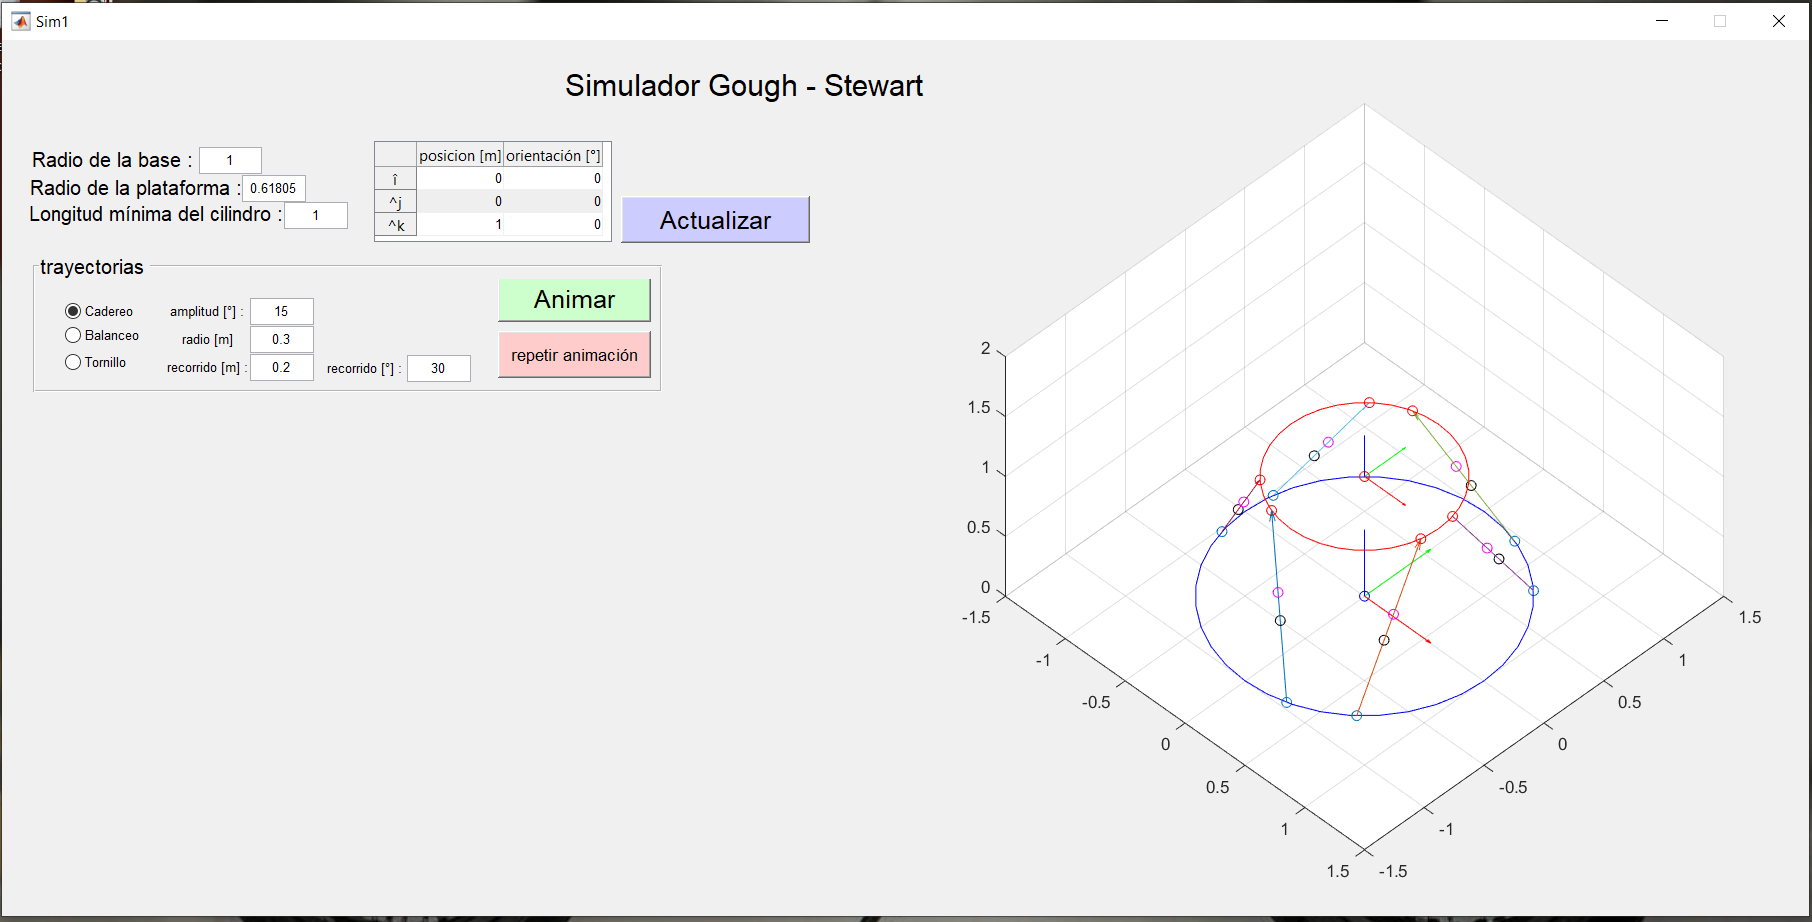
\includegraphics[scale=0.2]{img/principal.png}
 % principal.png: 1812x922 px, 120dpi, 38.36x19.52 cm, bb=0 0 1087 553
 \caption{Interfaz gráfica del simulador.}
 \label{fig: GUI}
\end{figure}


El simulador determina si la posición y 
orientación introducidas en la interfaz gráfica
es realizable con los parámetros especificados para
el robot. Para llegar a este resultado, el simulador realiza
las siguientes instrucciones:

\begin{itemize}
 \item Obtener la posición de cada junta de la base,
 con respecto al centro de la base.
 \item Obtener la posición de cada junta de la
 plataforma móvil con respecto a la base y tomando
 en cuenta la posición deseada.
 \item Procesar las coordenadas de cada elemento para 
 obtener los vectores que representan cada pistón.
 \item Evaluar si la posición deseada excede las 
 limitaciones físicas del sistema como exceder la 
 extensión o compresión máxima de algún pistón.
 \item Enviar mensajes de error si es necesario.
 \item Graficar los datos obtenidos, en caso de ser una
 posición factible.
 \item Ejcutar instrucciones adicionales 
 de la interfaz gráfica.
\end{itemize}

El simulador también es capaz de producir animaciones del 
movimiento de la plataforma y exportarlas como 
archivos MP4.


\section{Resultados}

Las estrategias de control implementadas fueron probadas con dos casos de prueba: bajo una referencia estática en un punto arbitrario y bajo el seguimiento de una trayectoria circular.

El caso bajo una referencia estática se evaluó el tiempo de estabilización y el error en estado estable y en el caso de seguimiento de trayectorias se evaluó qué tan robusto es el sistema y el comportamiento del mismo fuera del punto de linealización.

Los controles que fueron implementados 
\subsection{Control PD}

\subsubsection{Bajo patrón de movimiento}
\begin{figure}[h]
    \centering
    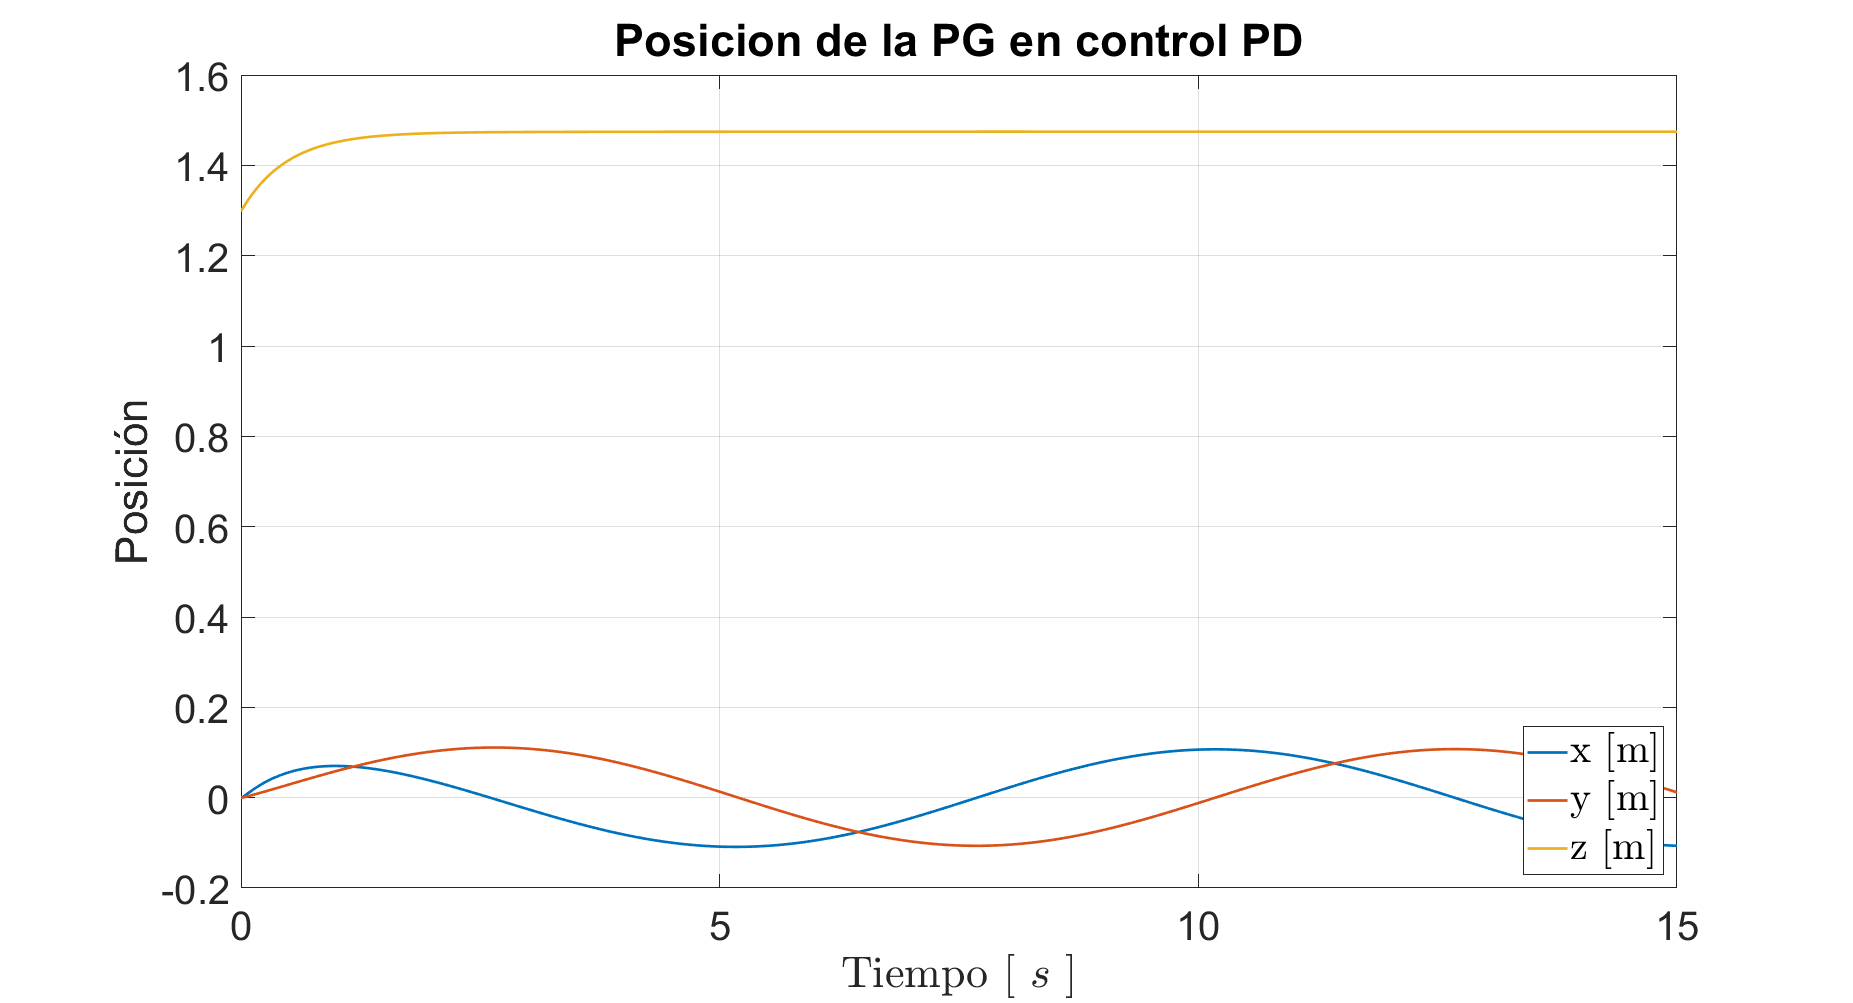
\includegraphics[width=0.4\textwidth]{posPD.png}
    \caption{Posición del sistema - PD.}
    \label{fig:PD position}
\end{figure}

\begin{figure}[h]
    \centering
    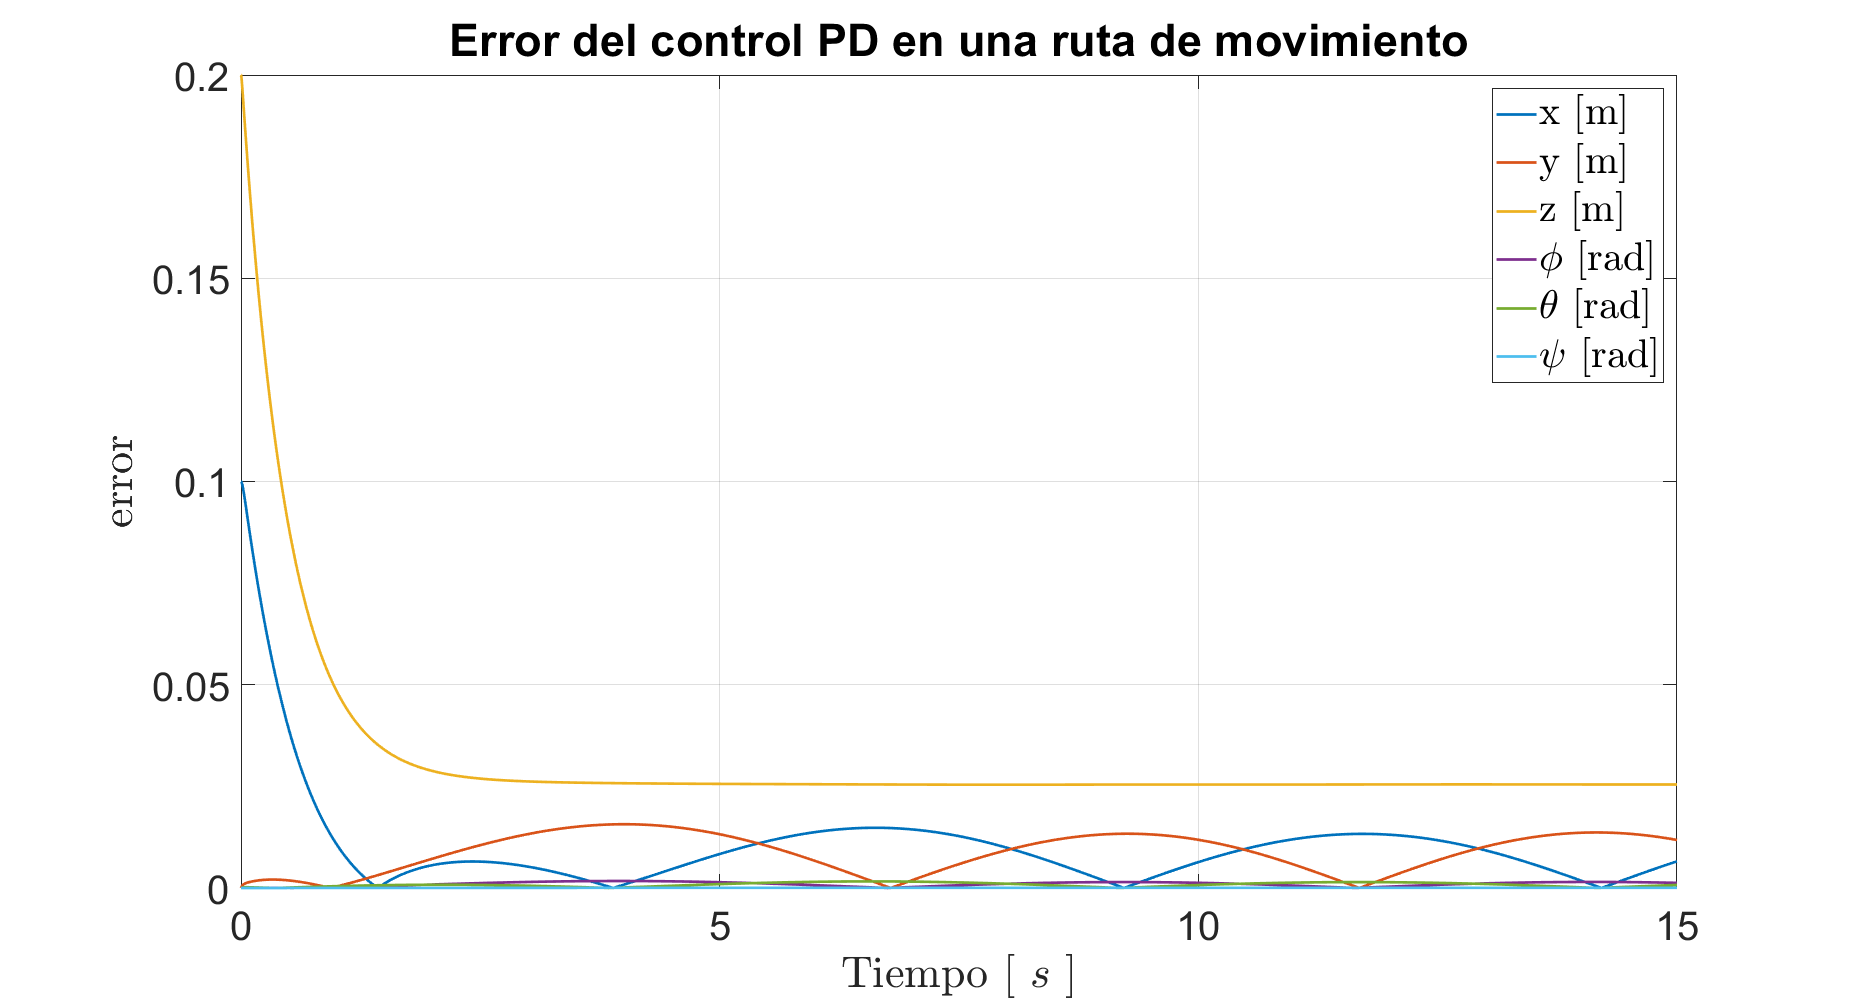
\includegraphics[width=0.4\textwidth]{errorPD.png}
    \caption{Error del sistema - PD.}
    \label{fig:PD error}
\end{figure}

\subsubsection{Bajo una referencia estática}

\begin{figure}[htb]
    \centering
    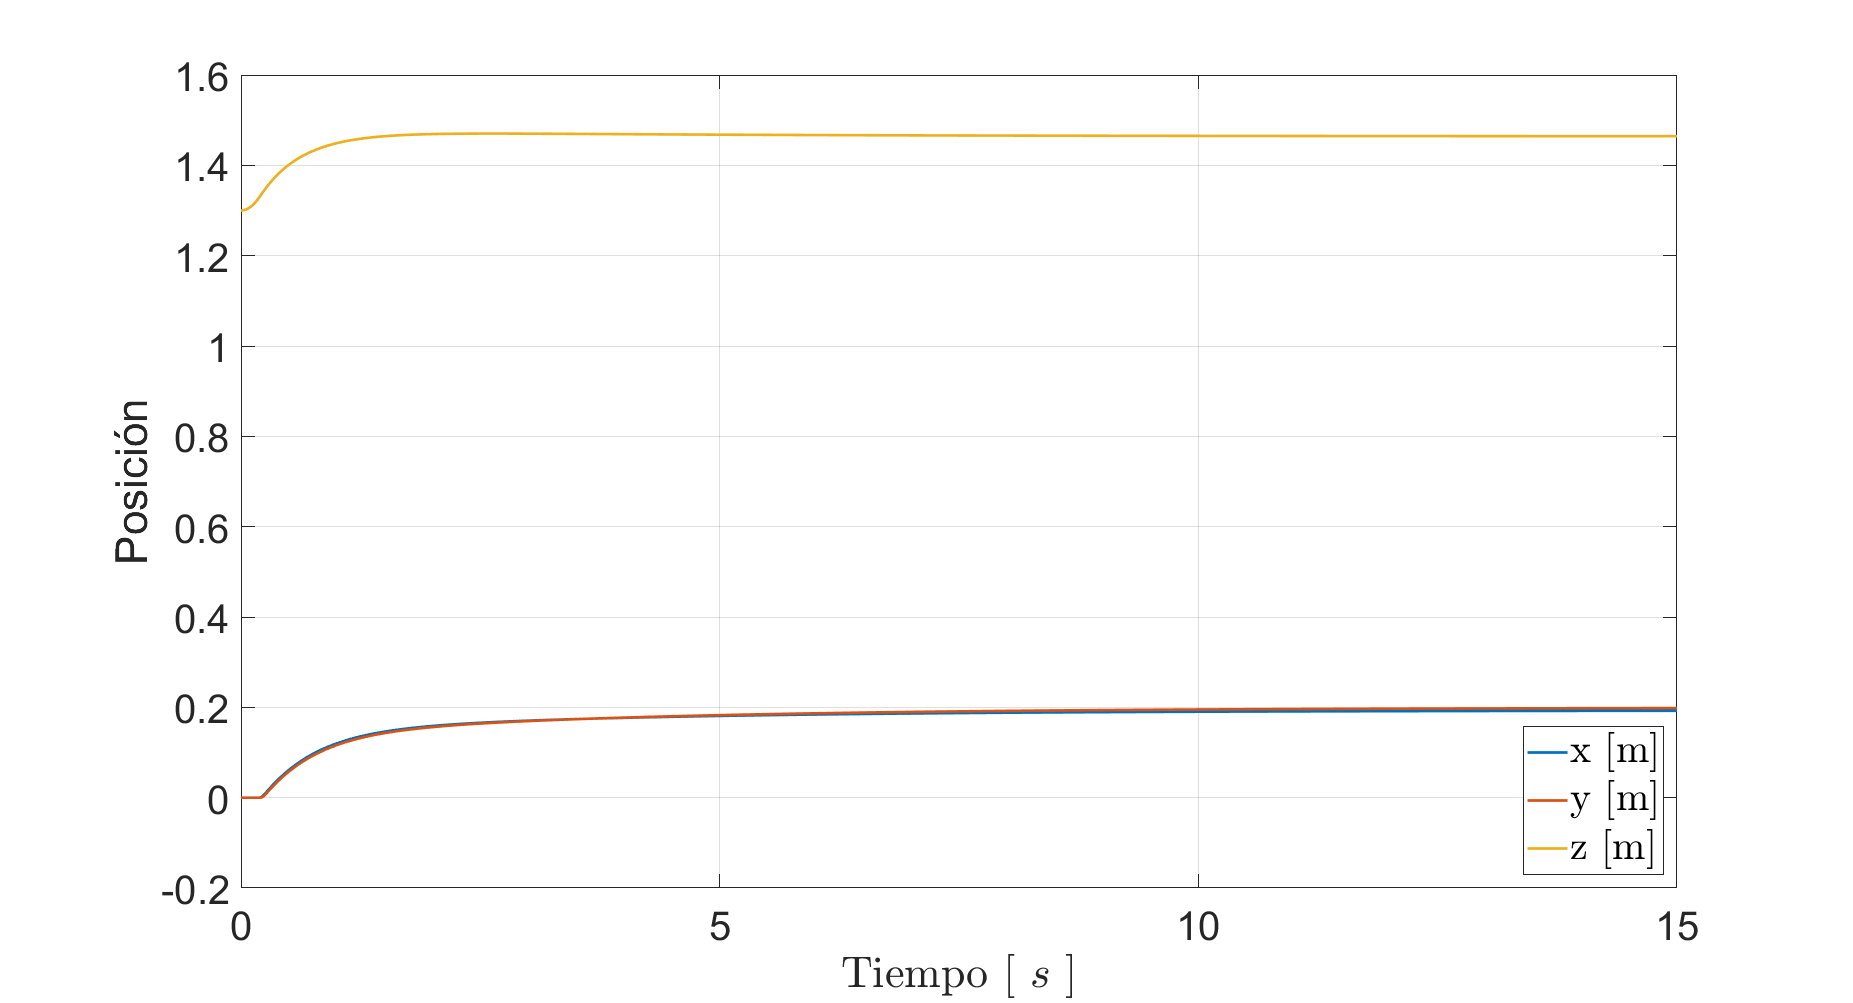
\includegraphics[width=0.4\textwidth]{posPDe.png}
    \caption{Posición del sistema - PD.}
    \label{fig:PD position}
\end{figure}

\begin{figure}[htb]
    \centering
    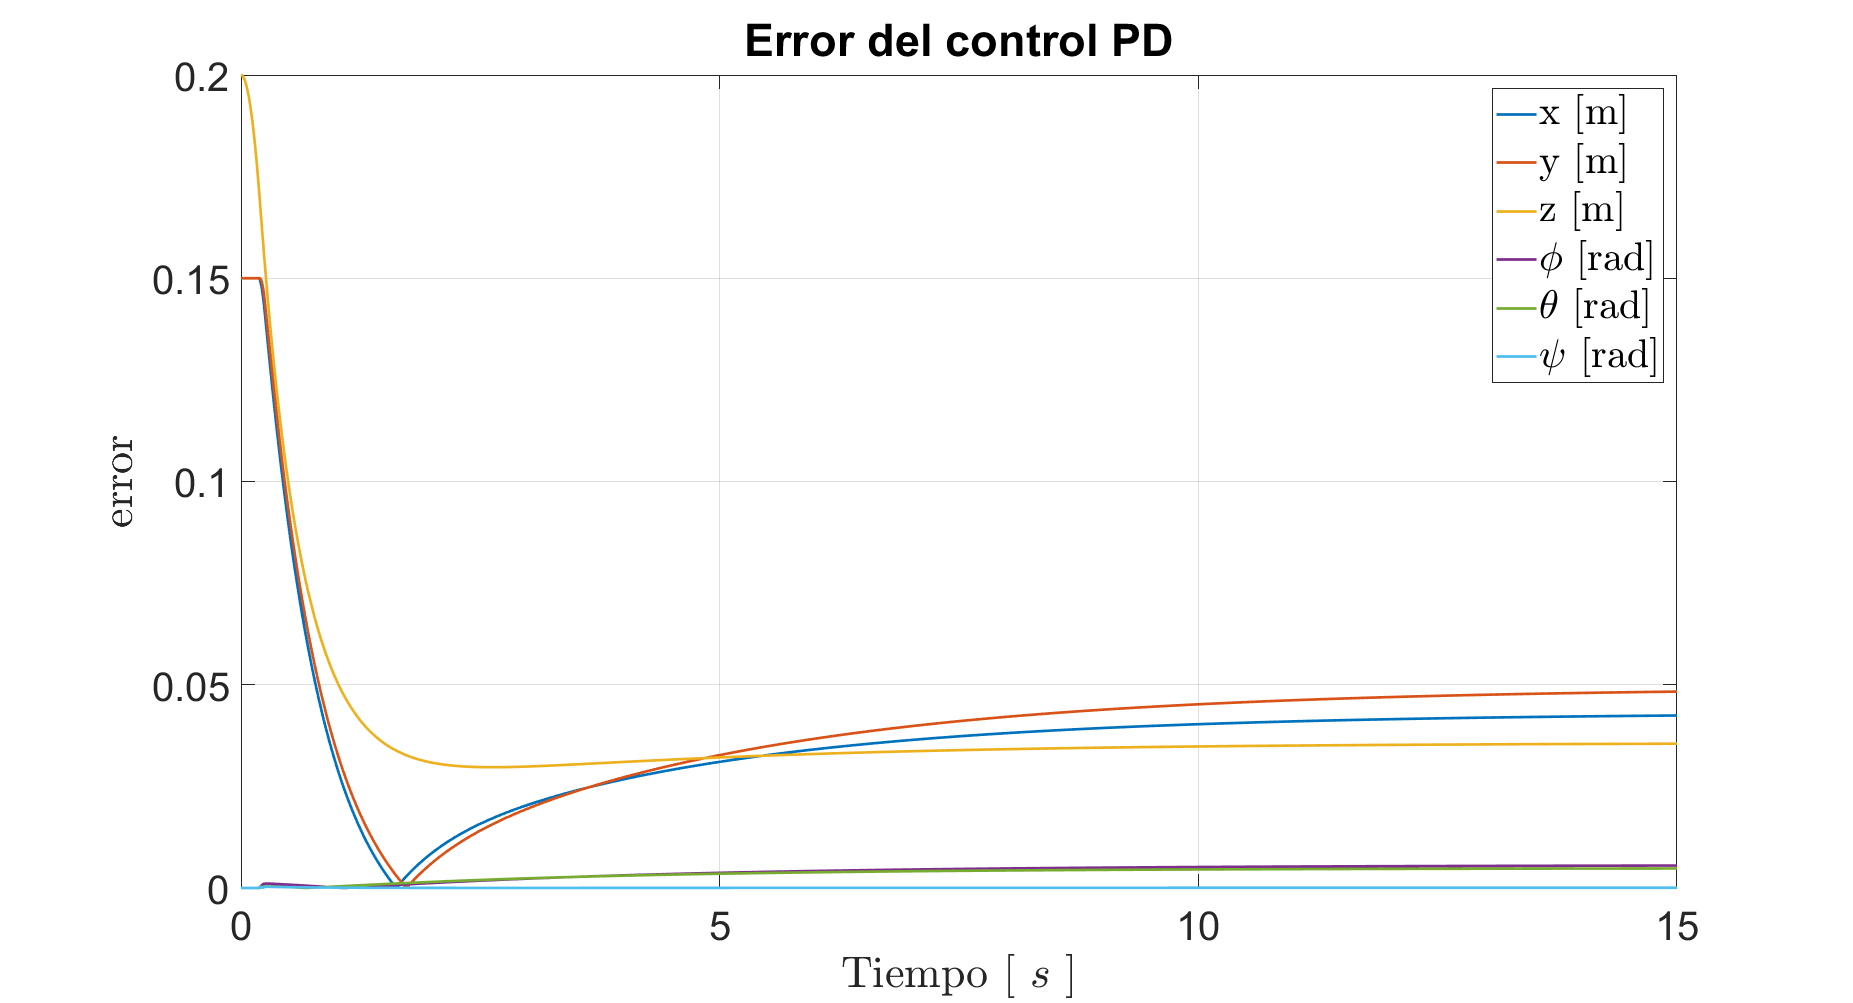
\includegraphics[width=0.4\textwidth]{errorPDe.png}
    \caption{Error del sistema - PD.}
    \label{fig:PD error}
\end{figure}


\subsection{Control PD+G}

\subsubsection{Bajo patrón de movimiento}

\begin{figure}[htb]
    \centering
    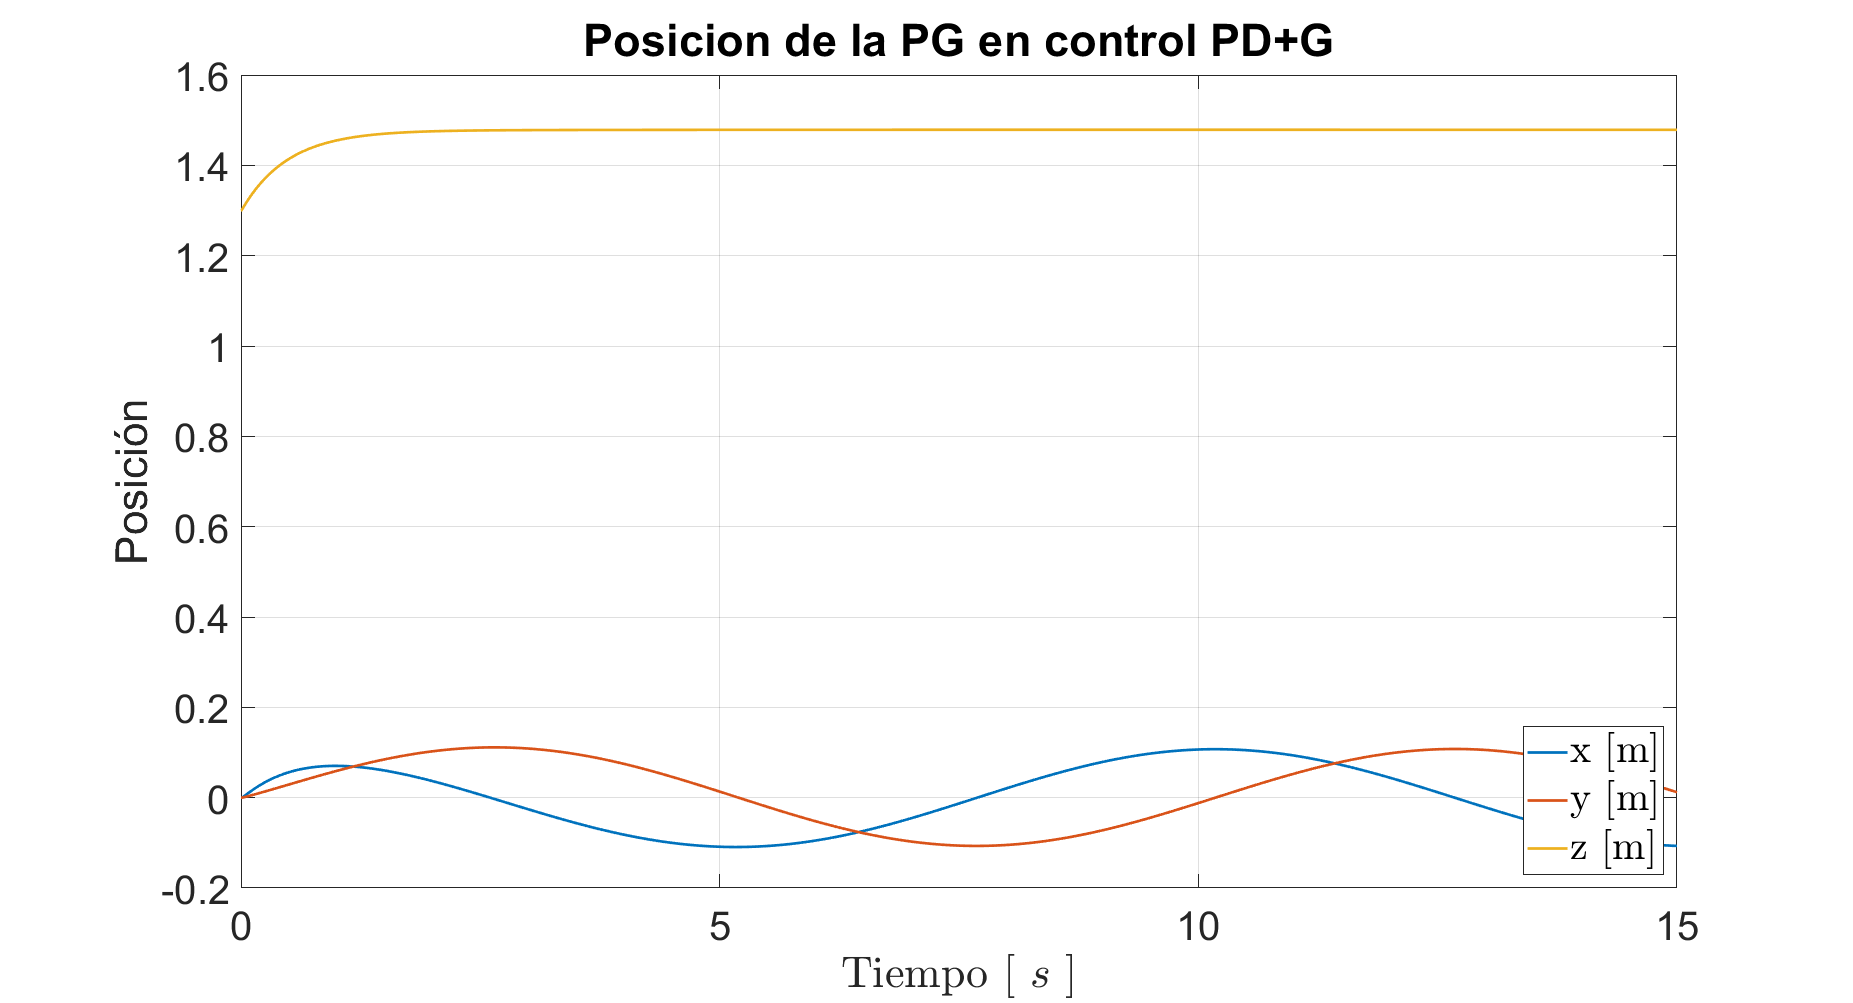
\includegraphics[width=0.4\textwidth]{posPDpG.png}
    \caption{Posición del sistema - PD+G.}
    \label{fig:PDG position}
\end{figure}

\begin{figure}[htb]
    \centering
    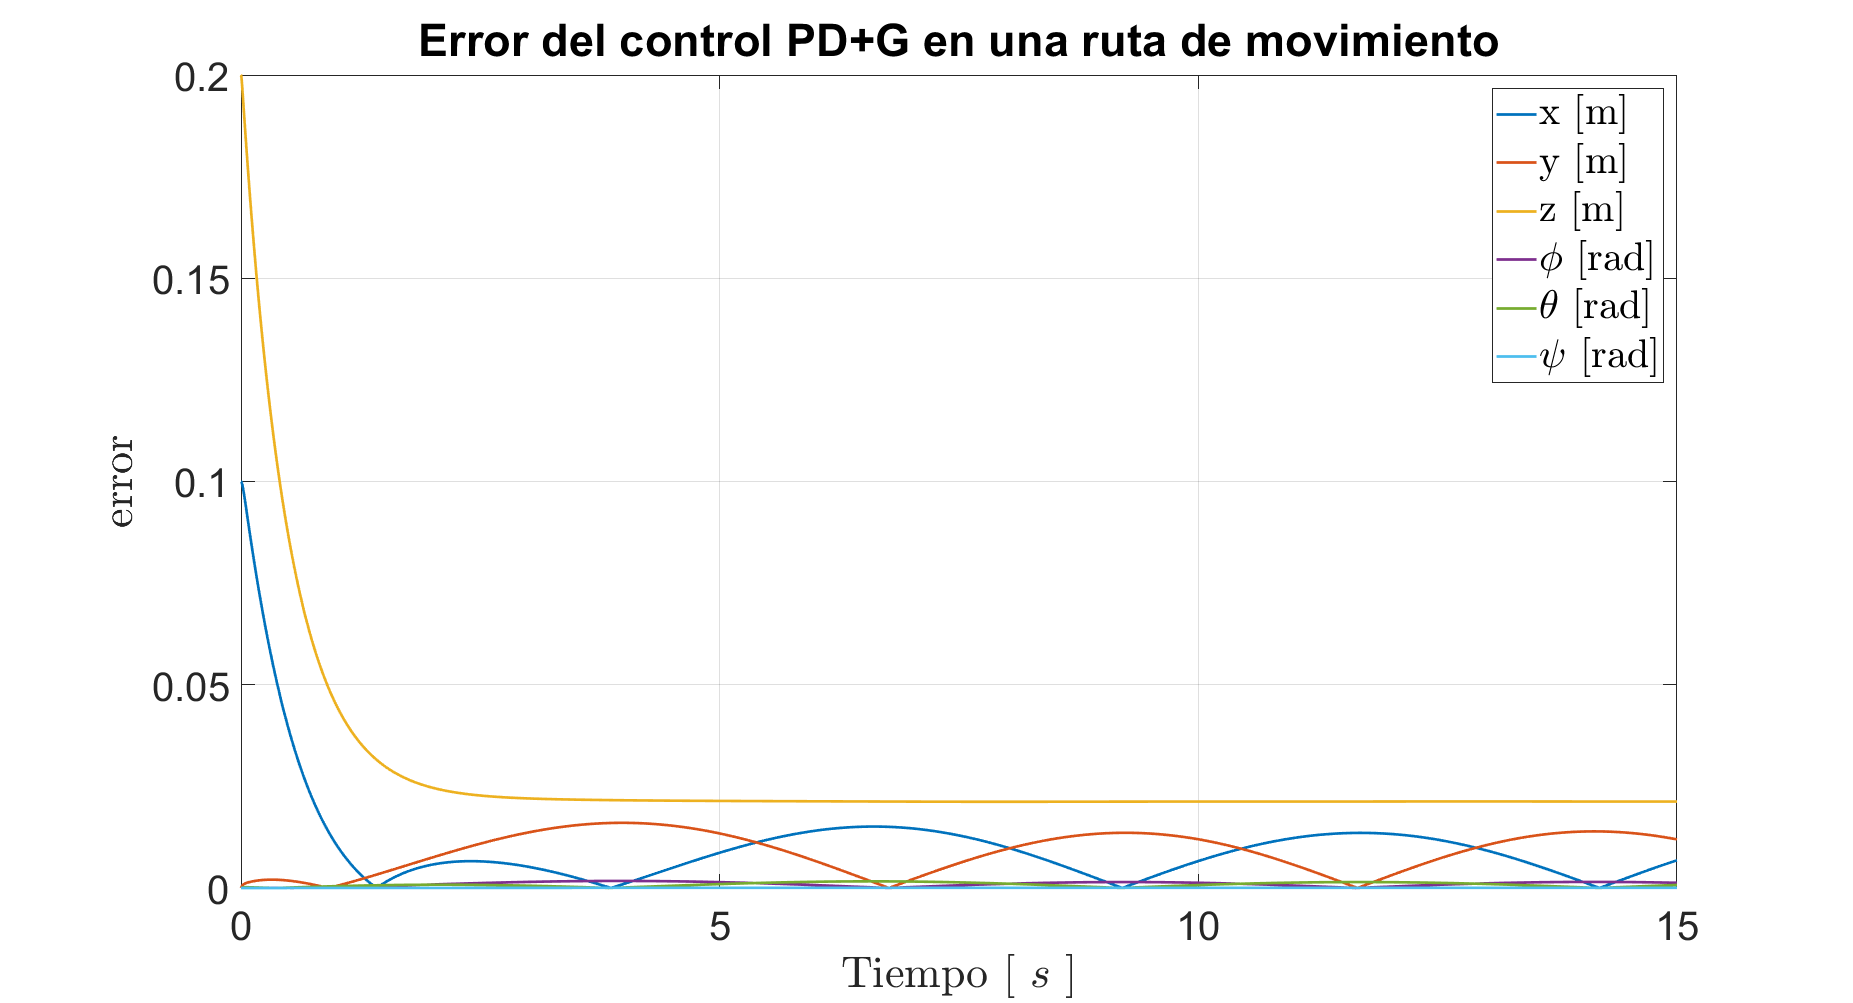
\includegraphics[width=0.4\textwidth]{errorPDpG.png}
    \caption{Error del sistema - PD+G.}
    \label{fig:PDG error}
\end{figure}

\subsubsection{Bajo una referencia estática}

\begin{figure}[htb]
    \centering
    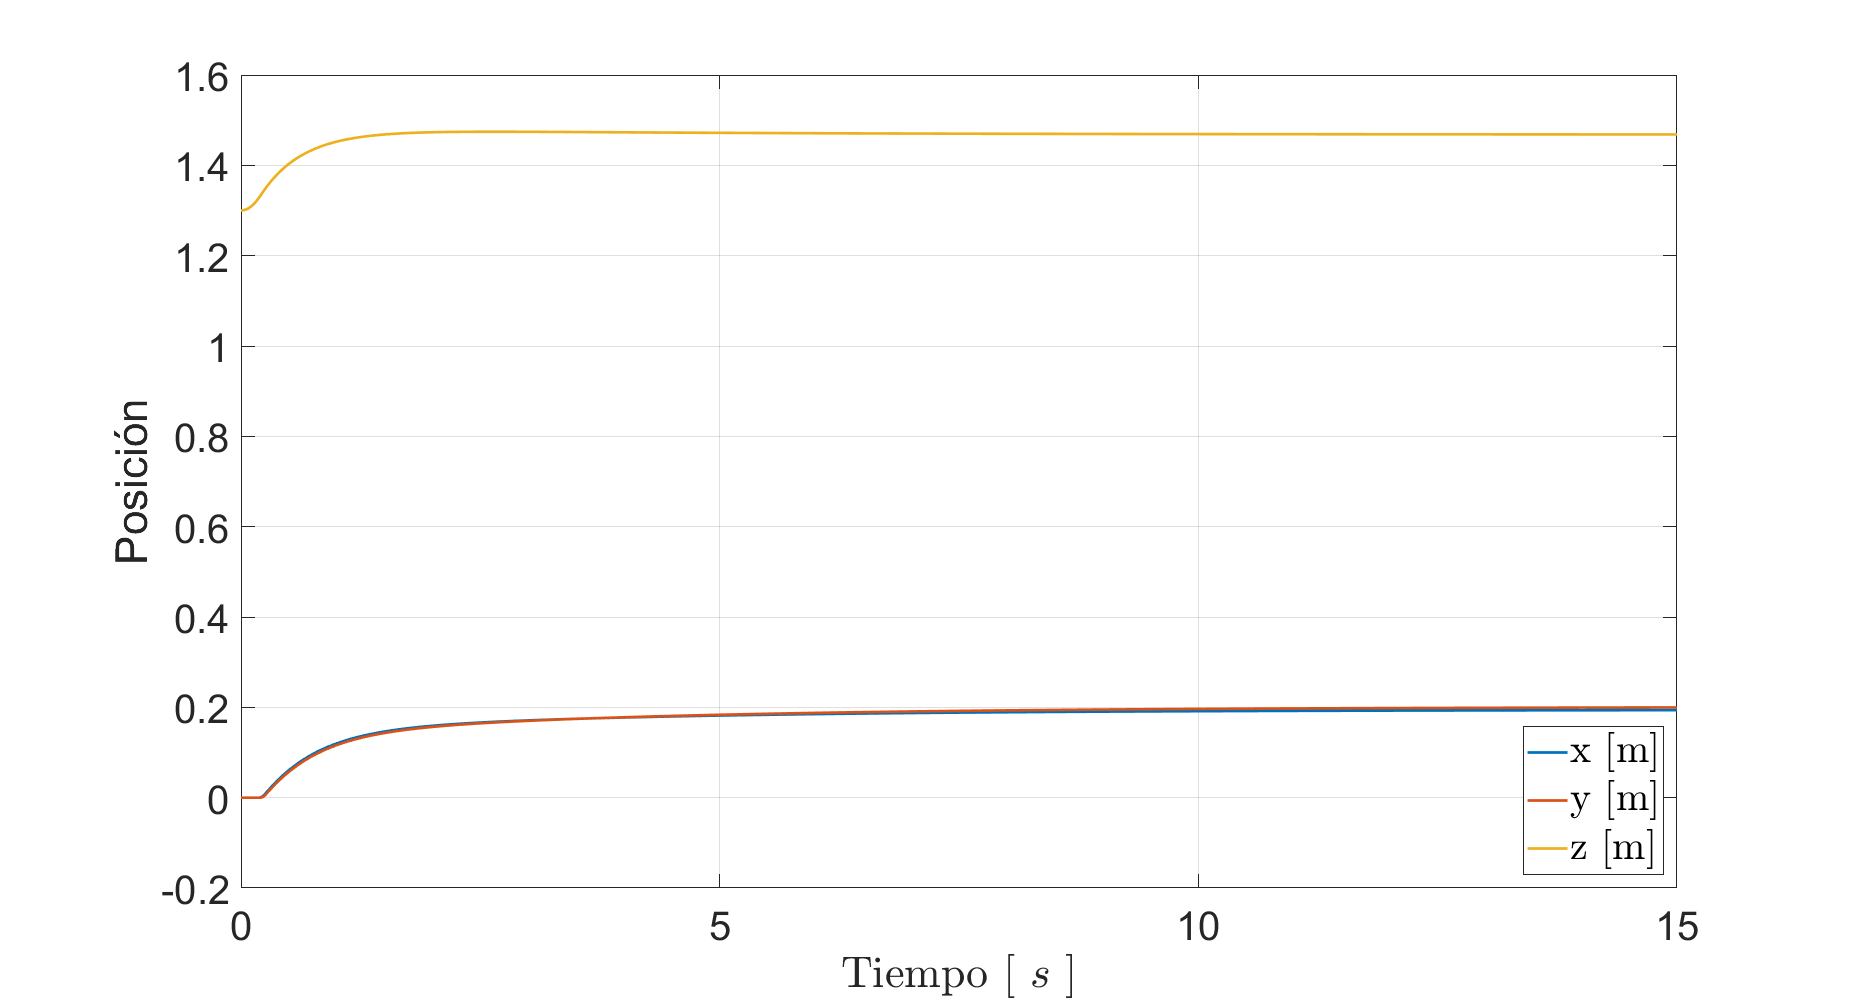
\includegraphics[width=0.4\textwidth]{posPDpGe.png}
    \caption{Posición del sistema - PD+G.}
    \label{fig:PDG position}
\end{figure}

\begin{figure}[htb]
    \centering
    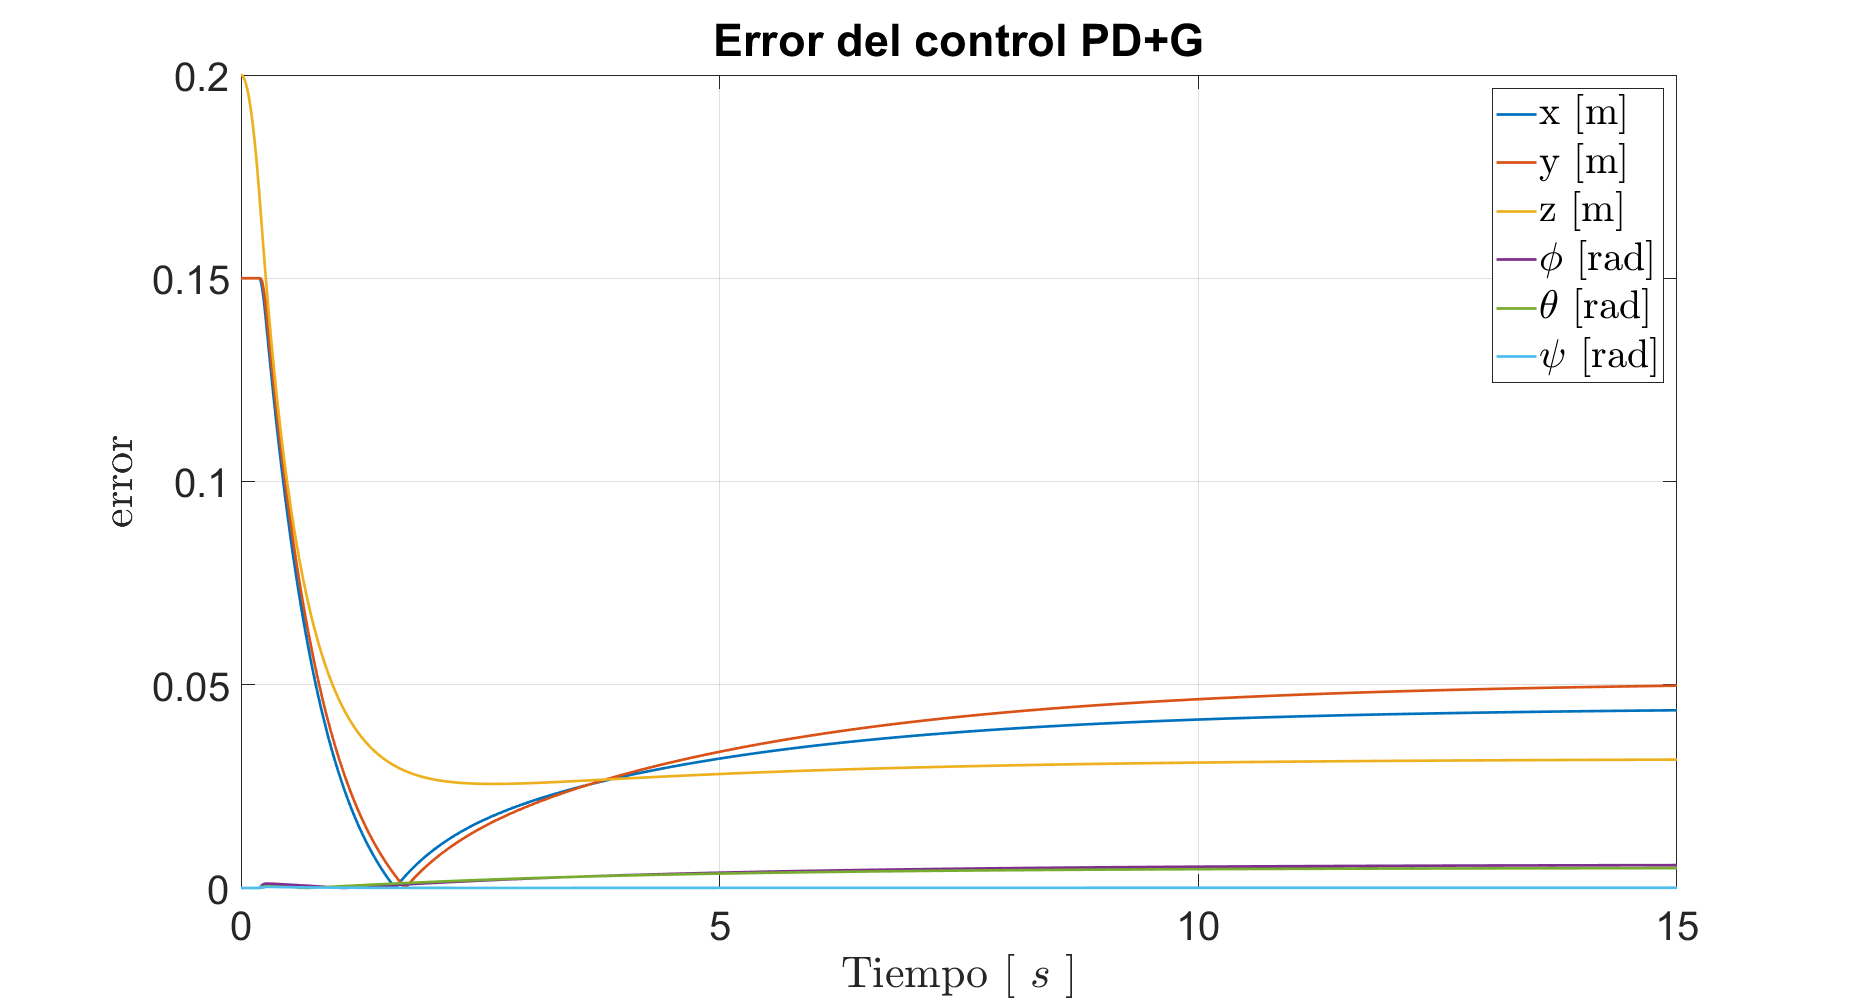
\includegraphics[width=0.4\textwidth]{errorPDpGe.png}
    \caption{Error del sistema - PD+G.}
    \label{fig:PDG error}
\end{figure}


\subsection{Control PID}

\subsubsection{Bajo patrón de movimiento}

\begin{figure}[htb]
    \centering
    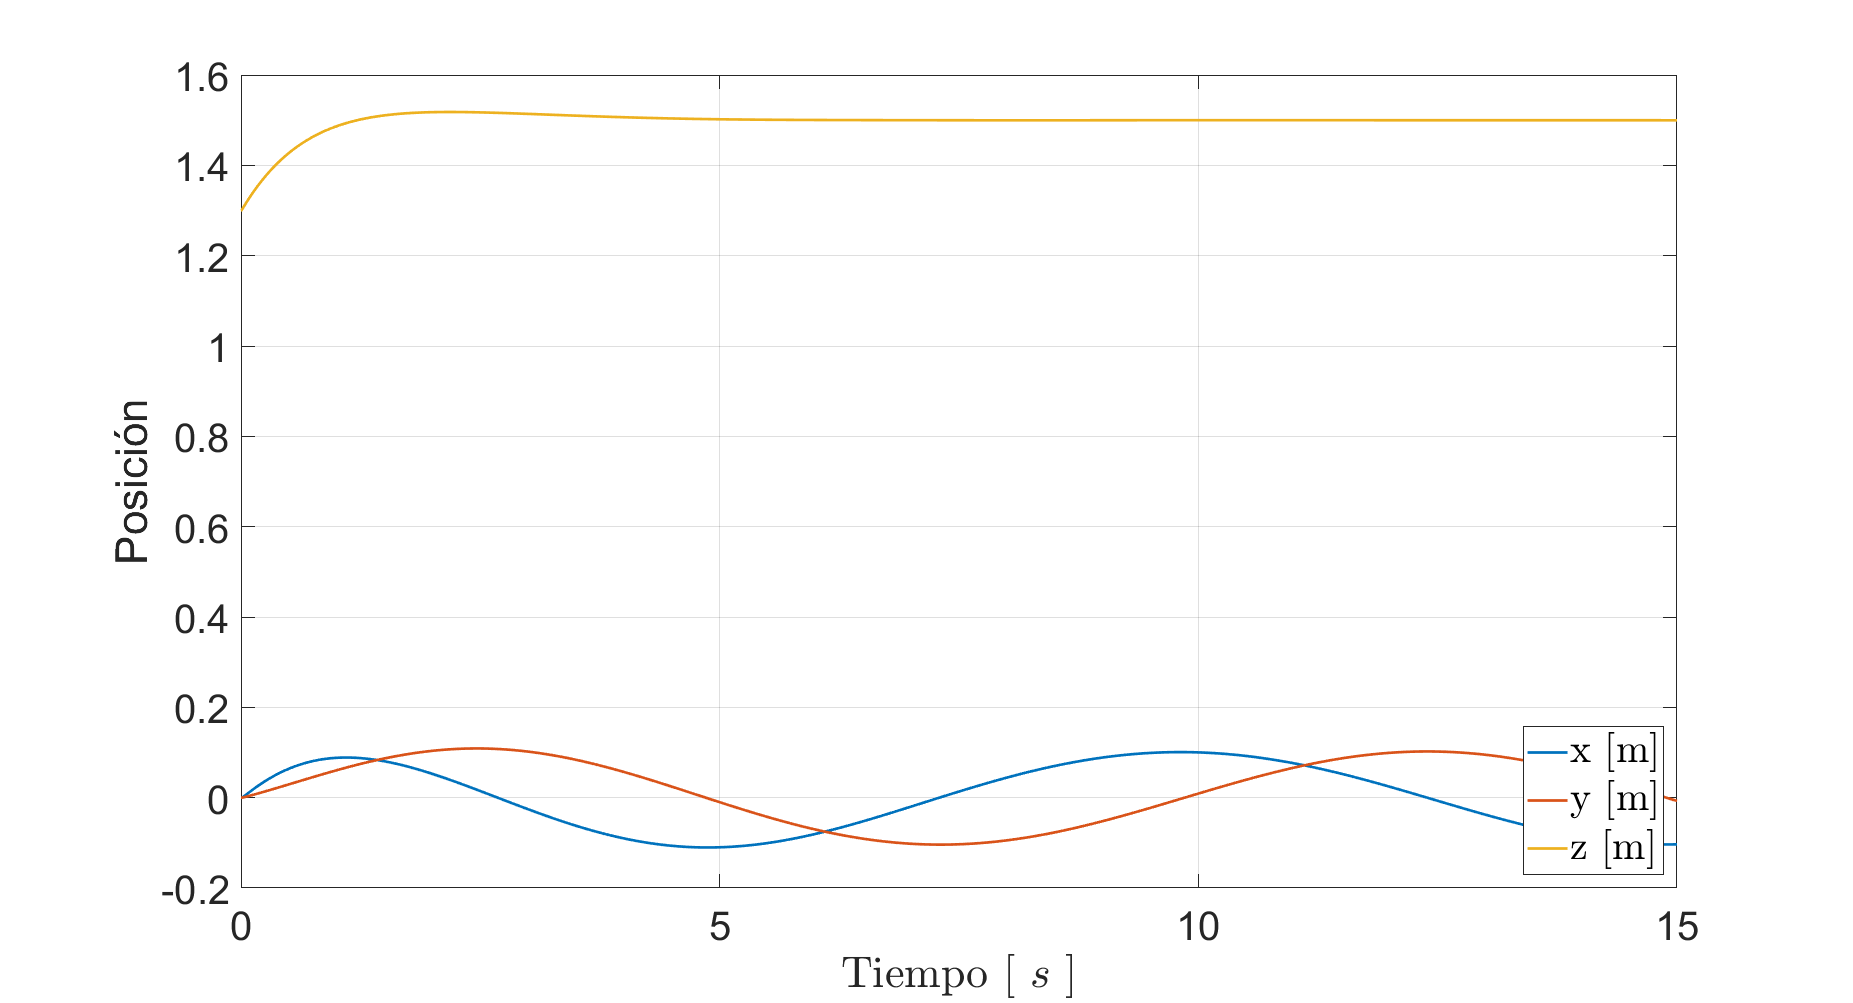
\includegraphics[width=0.4\textwidth]{posPID.png}
    \caption{Posición del sistema - PID.}
    \label{fig:PID position}
\end{figure}

\begin{figure}[htb]
    \centering
    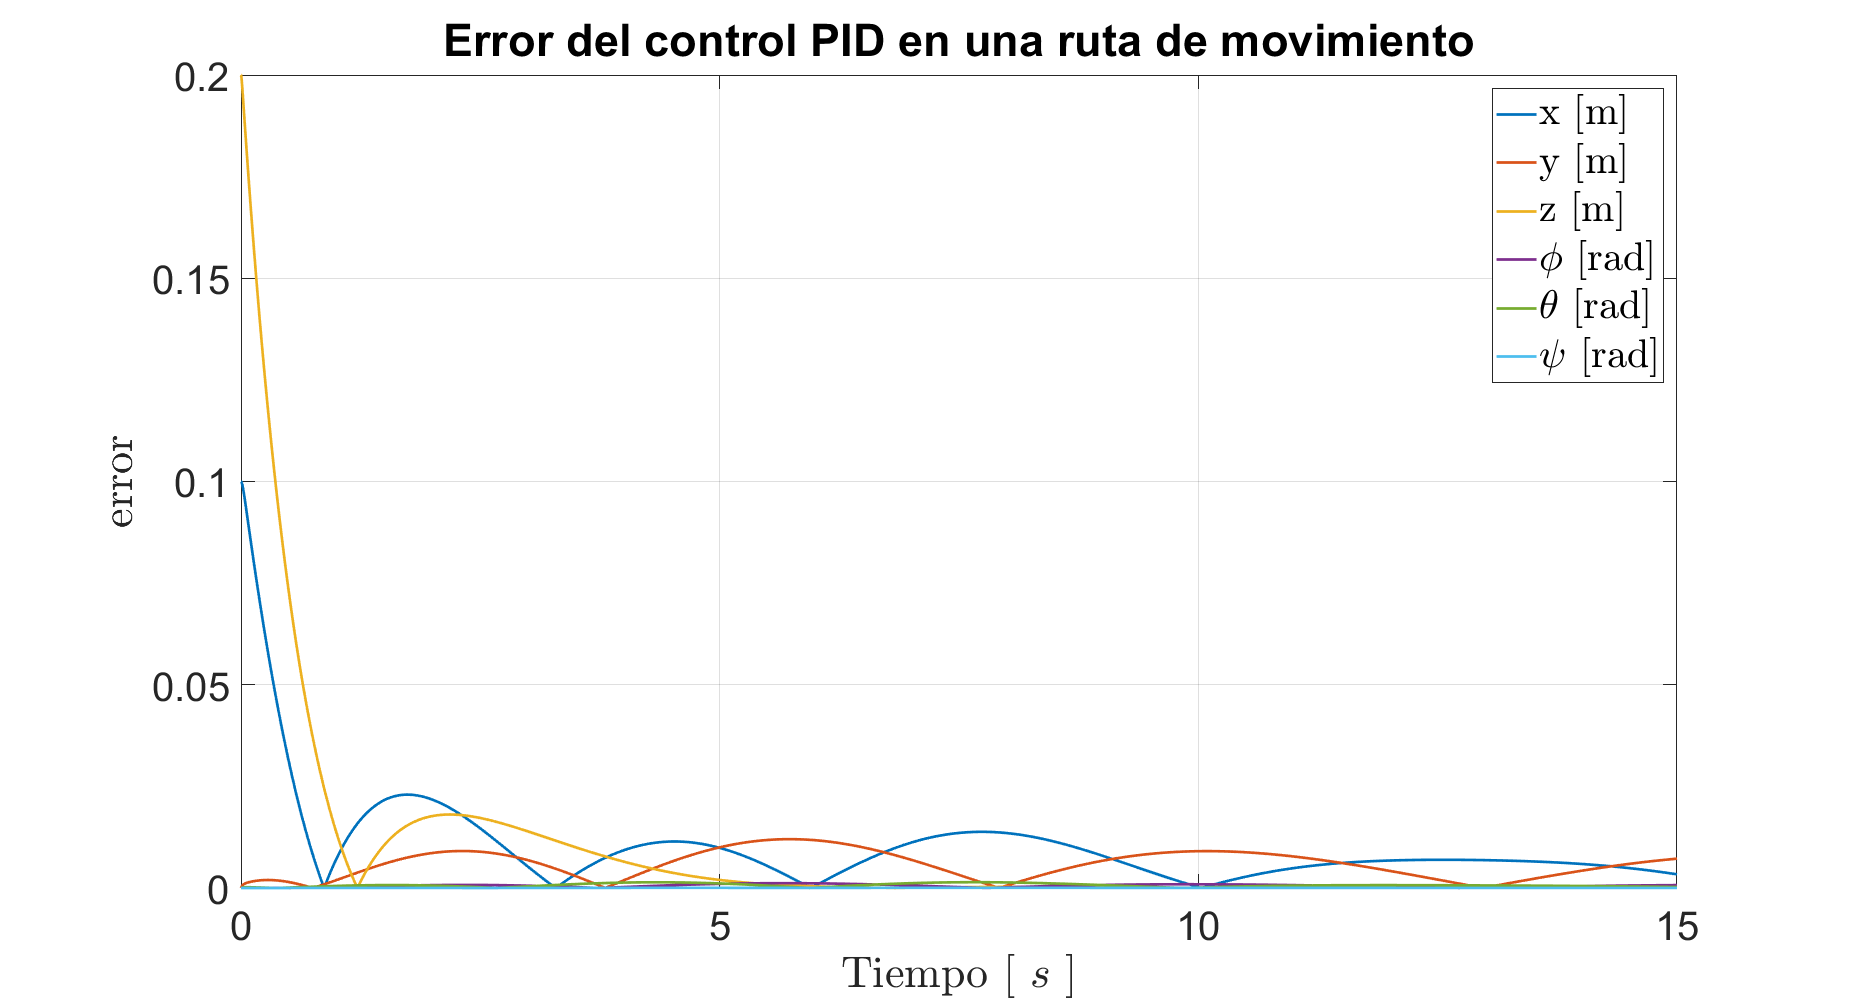
\includegraphics[width=0.4\textwidth]{errorPID.png}
    \caption{Error del sistema - PID.}
    \label{fig:PID error}
\end{figure}

\subsubsection{Bajo una referencia estática}

\subsubsection{Bajo patrón de movimiento}

\begin{figure}[htb]
    \centering
    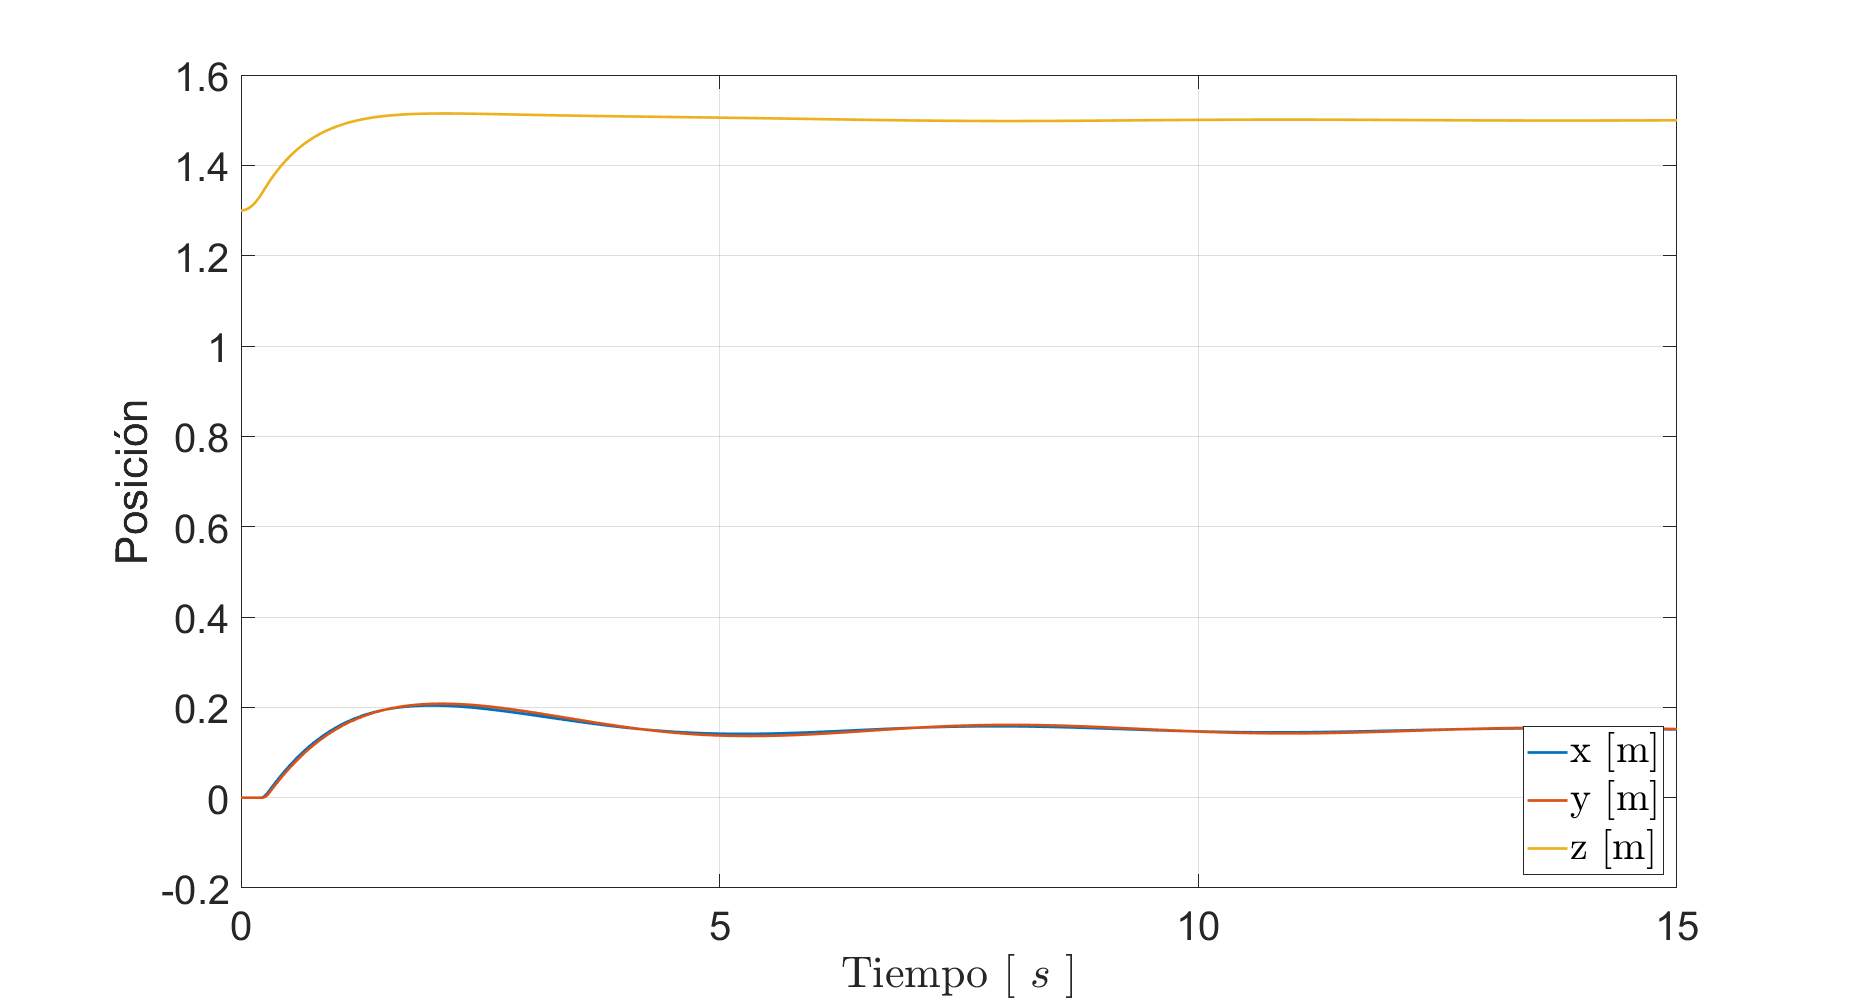
\includegraphics[width=0.4\textwidth]{posPIDe.png}
    \caption{Posición del sistema - PID.}
    \label{fig:PID position}
\end{figure}

\begin{figure}[htb]
    \centering
    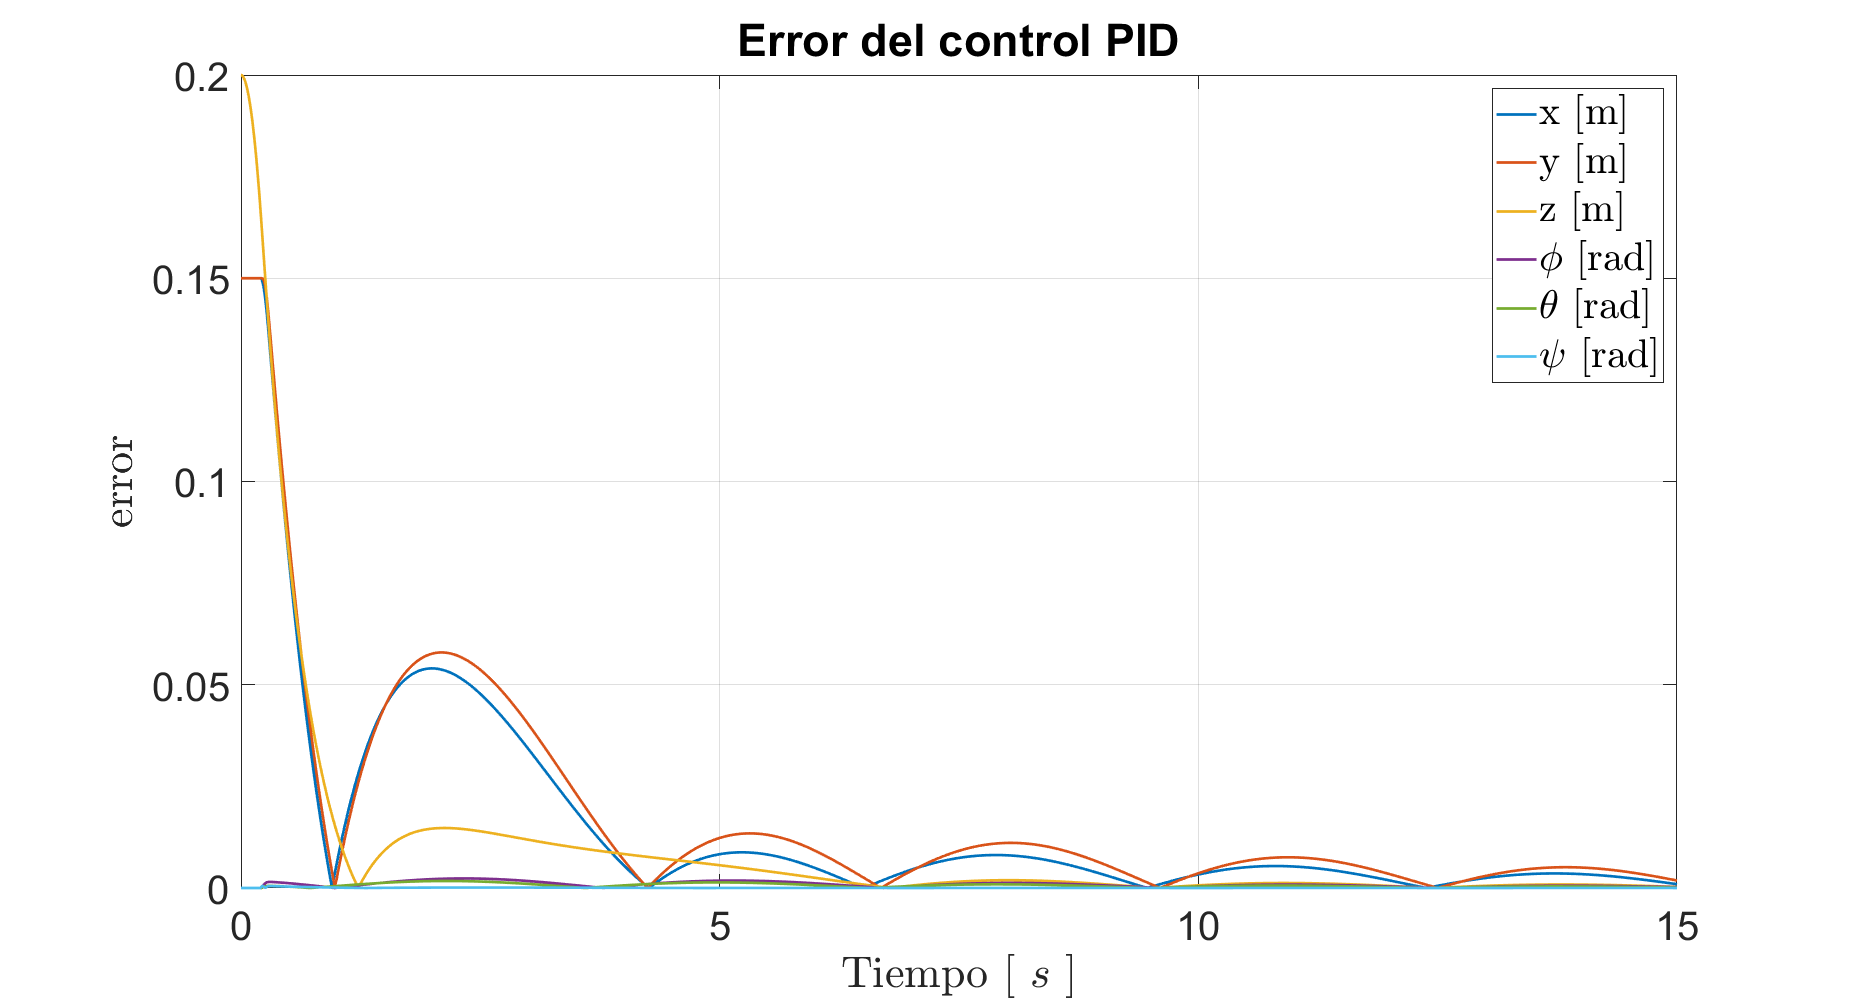
\includegraphics[width=0.4\textwidth]{errorPIDe.png}
    \caption{Error del sistema - PID.}
    \label{fig:PID error}
\end{figure}
\section{Discusión}

\subsection{Entendimiento del problema}

\subsection{Simulador en lazo abierto}

\subsection{Implementación de estrategias de control}



\subsection{Implementación de resortes de fin de carrera}




\bibliographystyle{IEEEtran}
\bibliography{bibliografia.bib}

% \pagebreak

\begin{appendices}
\section{Momentos de inercia}
\label{sec: inertia}

Los momentos de inercia del sistema fueron obtenidos
empleando la herramienta de Solidworks. 
Las propiedades de densidad de los componentes 
fueron asignados de acuerdo al material de manufactura
\footnote{El motor se asume como una masa uniformemente distribuida.}.

El tensor de inercia de cada objeto fue medido respecto a su centro de masa.
Empleando el teorema de ejes paralelos 
\cite{olguin20183d}
se trasladó el efecto de los tensores de inercia necesarios al marco referencial local.
A continuación se presentan los valores correspondientes a cada objeto de interés para la simulación.

El tensor de inercia se obtiene de la combinación lineal 
de los componentes $P_x$, $P_y$ y $P_z$ y los vectores $\mathbf I_x$, $\mathbf I_y$, e $\mathbf I_z]$.
Se realiza también la conversión adecuada de unidades al
sistema internacional.

\begin{equation*}
 I = abs(P_x \mathbf I_x) + abs(P_y \mathbf I_y) +abs(P_z \mathbf I_z)
\end{equation*}

\subsection{Plataforma móvil}

\begin{figure}[htb!]
    \centering
    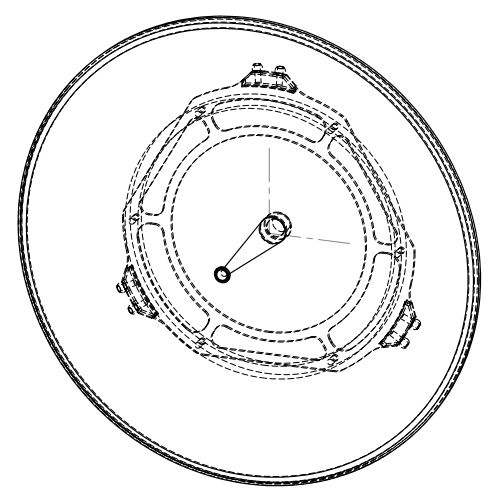
\includegraphics[width=8cm]{plat_D.JPG}
    \caption{Plataforma móvil.}
    \label{fig: cad platform}
\end{figure}

\begin{table}[hb!]
 \begin{center}
\begin{tabular}{lclc}
 Masa & $  115.53766 \ [kg]$ & $r_{cm}$ &  $[0; 0; 0.11145]^T \ [m]$ \\
 \hline
 & & & $[g/mm^2]$\\
 \hline
 $ I_x $ & $ [1 \ 0 \ 0]^T $ & $ P_x $ & 7246289714.88\\
 $ I_y $ & $ [0 \ 1 \ 0]^T $ & $ P_y $ & 7246289714.88\\
 $ I_z $ & $ [0 \ 0 \ 1]^T $ & $ P_z $ & 13887070726.86
\end{tabular}
\end{center}
\caption{Datos de inercia de la plataforma móvil.}
\label{tab: inertia table platform}
\end{table}


\subsection{Base}
\begin{figure}[htb!]
    \centering
    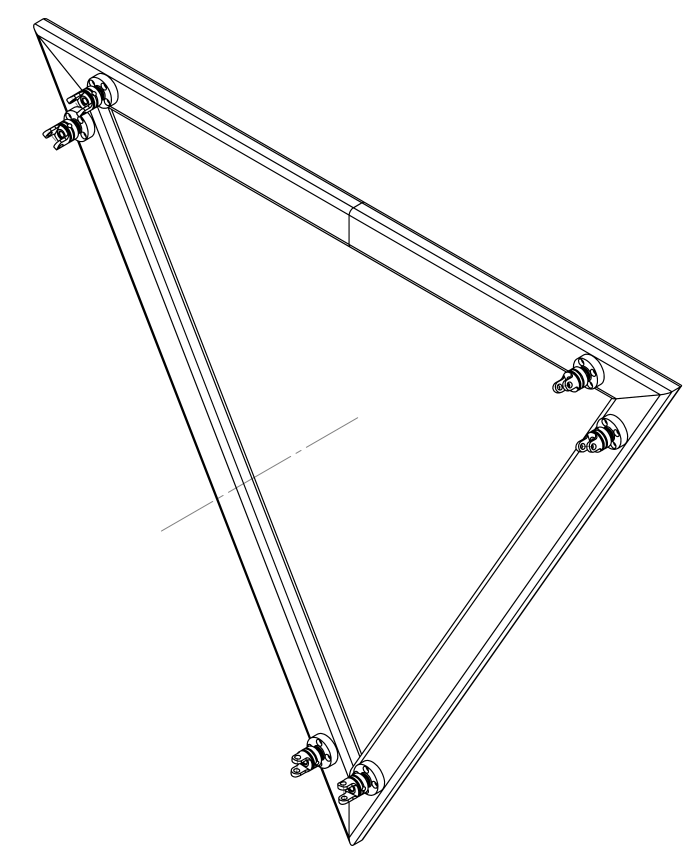
\includegraphics[width=8cm]{BASE.png}
    \caption{Base del robot.}
    \label{fig: cad base}
\end{figure}
% Px = convertGramMM2toKgM2 * 348997674.08;
% Py = convertGramMM2toKgM2 * 349004086.28;
% Pz = convertGramMM2toKgM2 * 696714510.70;
% 
% Ix = [0.73; -0.68; 0];
% Iy = [0.68; 0.73; 0];
% Iz = [0; 0; 1.0];

\begin{table}[hb!]
 \begin{center}
\begin{tabular}{lclc}
 Masa & $ 5.44739\ [kg]$ & $r_{cm}$ &  $[0; 0; 0.00048]^T \ [m]$ \\
 \hline
 & & & $[g/mm^2]$\\
 \hline
 $ I_x $ & $ [0.73\ -0.68\ 0]^T $ & $ P_x $ & 348997674.08\\
 $ I_y $ & $ [0.68\ 0.73\ 0]^T $ & $ P_y $ & 349004086.28\\
 $ I_z $ & $ [0 \ 0 \ 1]^T $ & $ P_z $ & 696714510.70
\end{tabular}
\end{center}
\caption{Datos de inercia de la base.}
\label{tab: inertia table base}
\end{table}

\subsection{Actuador prismático con motor}

\begin{figure}[htb!]
    \centering
    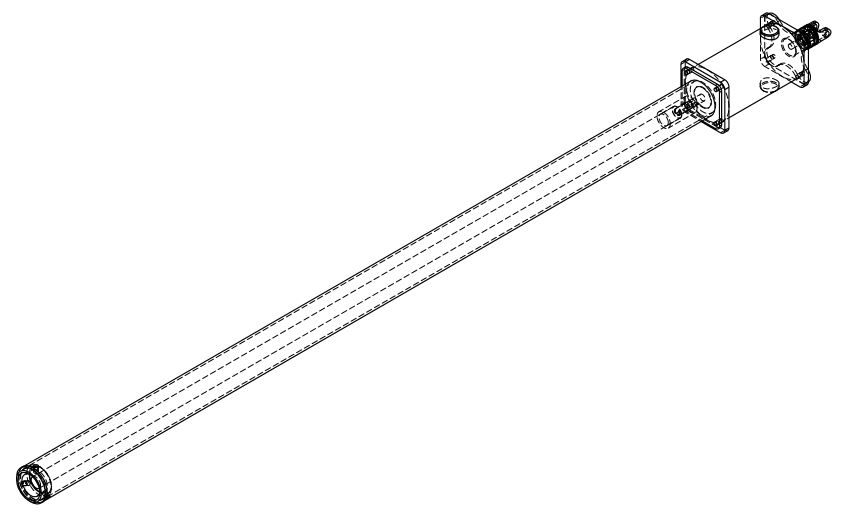
\includegraphics[width=8cm]{ACTUATOR.JPG}
    \caption{Actuador prismático.}
    \label{fig: cad motor}
\end{figure}

\begin{table}[hb!]
 \begin{center}
\begin{tabular}{lclc}


% Px = convertGramMM2toKgM2 * 2079848.97;
% Py = convertGramMM2toKgM2 * 703671034.55;
% Pz = convertGramMM2toKgM2 * 703687095.26;
% 
% Ix = [0; 0; 1];
% Iy = [0; -1; 0];
% Iz = [1; 0; 0];


 Masa & $ 5.48131 \ [kg]$ & $r_{cm}$ & $[0; 0; 0.47139]^T \ [m]$ \\
 \hline
 & & & $[g/mm^2]$\\
 \hline
 $ I_x $ & $ [0 \ 0 \ 1]^T $ & $ P_x $ & 2079848.97\\
 $ I_y $ & $ [0 \ -1 \ 0]^T $ & $ P_y $ & 703671034.55\\
 $ I_z $ & $ [1 \ 0 \ 0]^T $ & $ P_z $ & 703687095.26
\end{tabular}
\end{center}
\caption{Datos de inercia del actuador con motor.}
\label{tab: inertia table motor}
\end{table}

\subsection{Vástago con junta esférica}

\begin{figure}[htb!]
    \centering
    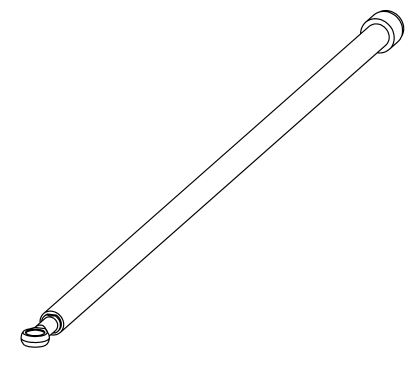
\includegraphics[width=8cm]{vastago_D.JPG}
    \caption{Vástago con junta esférica.}
    \label{fig:my_label}
\end{figure}

\begin{table}[hb!]
 \begin{center}
\begin{tabular}{lclc}


% Px = convertGramMM2toKgM2 * 297124.48;
% Py = convertGramMM2toKgM2 * 205340128.62;
% Pz = convertGramMM2toKgM2 * 205340128.62;
% 
% Ix = [0; 0; 1];
% Iy = [0.71; -0.71; 0];
% Iz = [0.71; 0.71; 0];

 Masa & $ 2.25414\ [kg]$ & $r_{cm}$ & $[0.00001; 0; -0.53696]^T \ [m]$  \\
 \hline
 & & & $[g/mm^2]$\\
 \hline
 $ I_x $ & $ [0 \ 0 \ 1]^T $ & $ P_x $ & 297124.48\\
 $ I_y $ & $ [0.71 \ -0.71 \ 0]^T $ & $ P_y $ & 205340128.62\\
 $ I_z $ & $ [0.71 \ 0.71 \ 0]^T $ & $ P_z $ & 205340128.62
\end{tabular}
\end{center}
\caption{Datos de inercia del vástago con junta esférica.}
\label{tab: inertia table joint}
\end{table}
 

\end{appendices}





% Se incluye como anexo los planos de la antena parabólica empleados para el 
% estudio de la dinámica
% de plataforma Gough Stewart, cortesía de la compañía \emph{radiowaves}\footnote{www.radiowaves.com}.



% 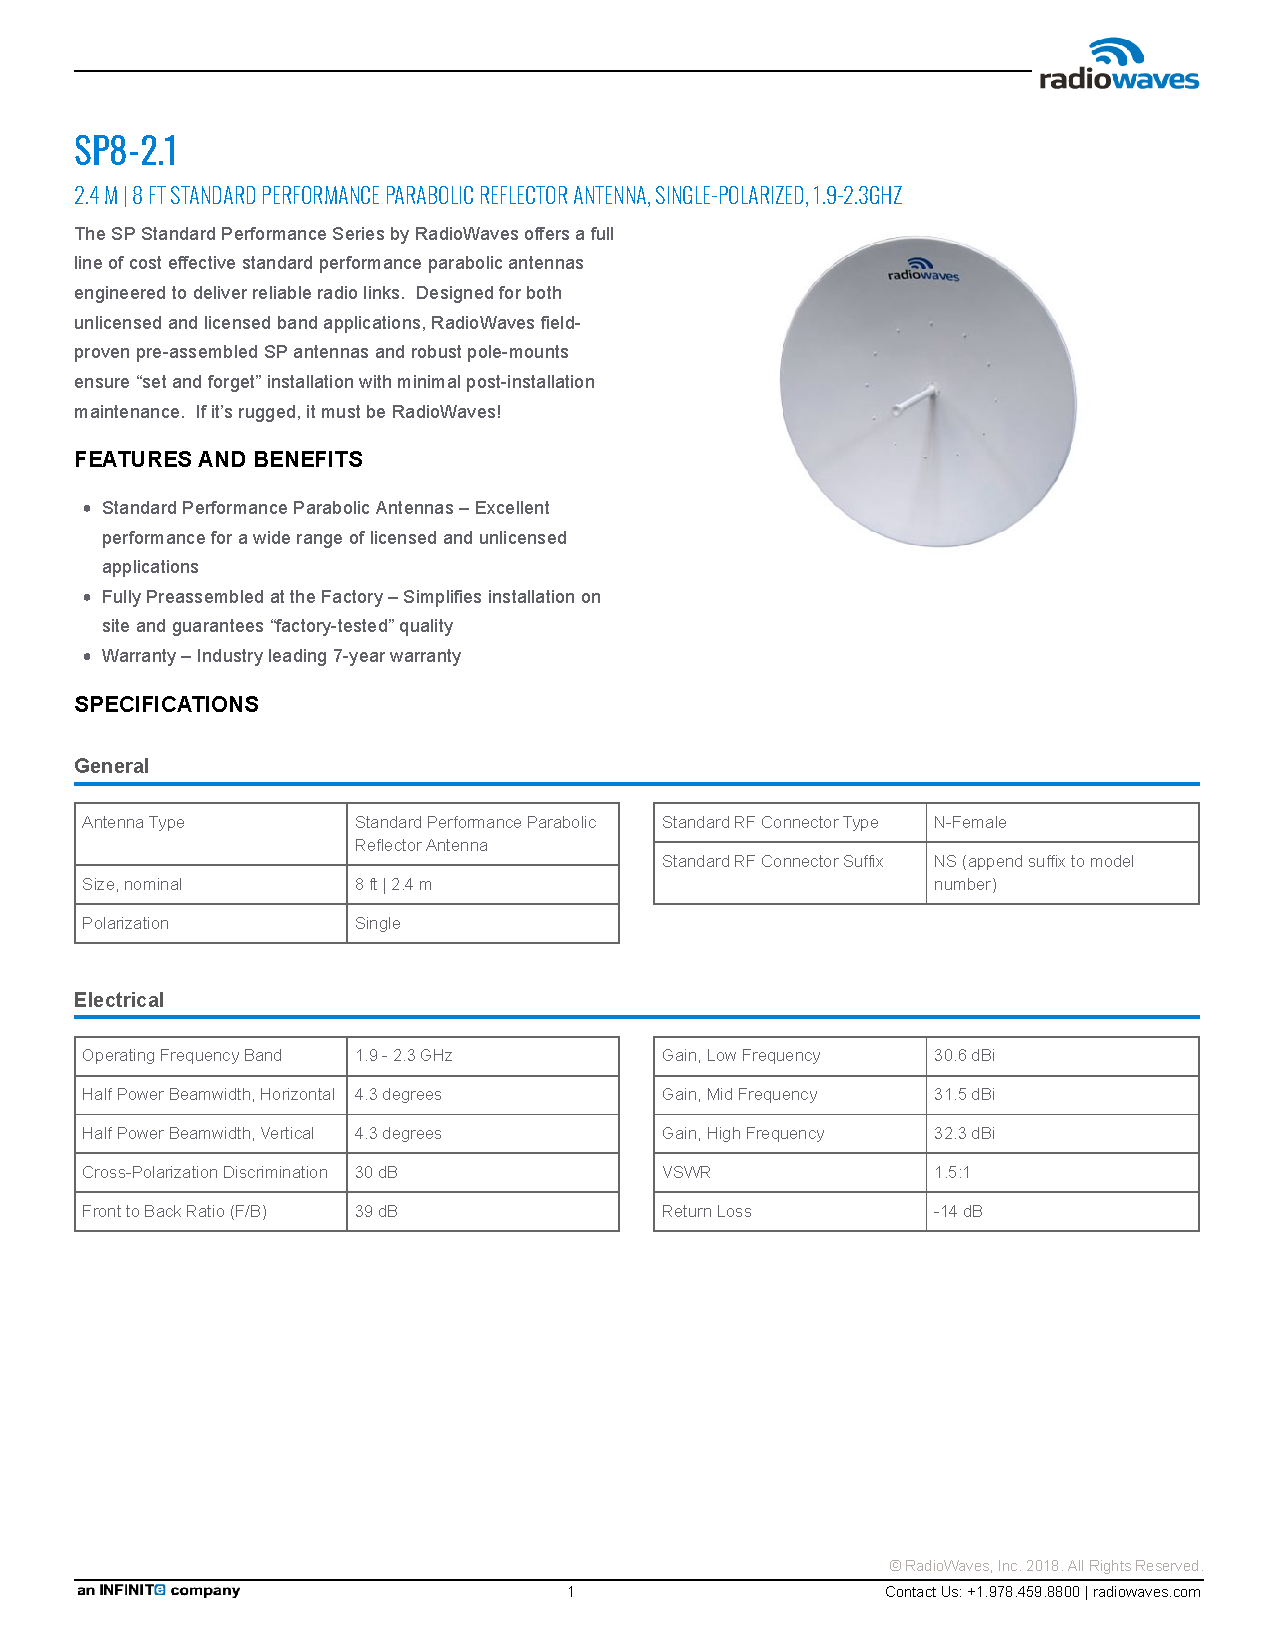
\includepdf[pagecommand={}, scale=1.0, pages={1,2,3}]{specs.pdf}


% \appendix
% \section{MATLAB}




\end{document}
